\documentclass[11pt,a4paper]{article}
\usepackage[utf8]{inputenc}
\usepackage[T1]{fontenc}
\usepackage[spanish,es-noshorthands]{babel}
\usepackage{geometry}
\geometry{margin=2.6cm}
\usepackage{calc}
\usepackage{longtable}
\usepackage{booktabs}
\usepackage{array}
\usepackage{ragged2e}
\usepackage{graphicx}
\usepackage{float}
\usepackage[table]{xcolor}
\usepackage{caption}
\captionsetup{skip=6pt}
\usepackage{titlesec}
\usepackage{fancyhdr}
\usepackage[hidelinks]{hyperref}
\usepackage{enumitem}
\usepackage{parskip}
\usepackage{needspace}
\usepackage{etoolbox}
\setlength{\parskip}{0.55em}
\setlist{itemsep=0.2em}

% evita titulos "huerfanos" solos al final de una pagina, empujandolos a la
% siguiente si no queda espacio para el titulo mas unas lineas de contenido
\pretocmd{\section}{\needspace{5\baselineskip}}{}{}
\pretocmd{\subsection}{\needspace{4\baselineskip}}{}{}
\pretocmd{\subsubsection}{\needspace{3\baselineskip}}{}{}

% --- Macros pandoc espera que existan (normalmente las inyecta su modo -s) ---
\providecommand{\tightlist}{%
  \setlength{\itemsep}{0pt}\setlength{\parskip}{0pt}}
\providecommand{\pandocbounded}[1]{#1}
\newcommand{\passthrough}[1]{#1}

\hypersetup{
  pdftitle={HemoScan Andino},
  pdfauthor={Equipo HemoScan Andino -- UPeU Juliaca},
  colorlinks=false,
  bookmarksopen=true
}

% El contenido ya trae su propia numeracion manual (1., 1.1, 1.1.1...) escrita
% en el texto de cada encabezado, asi que se desactiva la numeracion automatica
% de LaTeX para evitar una doble numeracion en el indice y en el cuerpo.
\setcounter{secnumdepth}{-2}
\setcounter{tocdepth}{4}
\titleformat{\section}{\normalfont\Large\bfseries}{}{0em}{}
\titleformat{\subsection}{\normalfont\large\bfseries}{}{0em}{}
\titleformat{\subsubsection}{\normalfont\normalsize\bfseries}{}{0em}{}

% Encabezado con dos etiquetas CORTAS y de ancho fijo (nunca texto largo o
% dinamico por subseccion) para que jamas puedan solaparse entre si.
\pagestyle{fancy}
\fancyhf{}
\fancyhead[L]{\small HemoScan Andino}
\fancyhead[R]{\small Entregable 1 --- Diagn\'ostico}
\fancyfoot[C]{\thepage}
\renewcommand{\headrulewidth}{0.4pt}

\begin{document}

\begin{titlepage}
\centering
\vspace*{1.2cm}
{\large UNIVERSIDAD PERUANA UNI\'ON\par}
{\normalsize Facultad de Ingenier\'ia y Arquitectura\par}
{\normalsize Escuela Profesional de Ingenier\'ia de Sistemas --- Filial Juliaca\par}
\vspace{0.5cm}
\rule{0.6\linewidth}{0.4pt}
\vspace{1.6cm}

{\large PROYECTO DE TESIS / PROYECTO INTEGRADOR\par}
\vspace{1.0cm}
{\huge\bfseries HemoScan Andino\par}
\vspace{0.6cm}
{\Large Sistema no invasivo de tamizaje de anemia infantil con fusi\'on \'optica multisensor y autocalibraci\'on por altitud\par}
\vspace{1.6cm}
\rule{0.6\linewidth}{0.4pt}
\vspace{1.6cm}

{\Large\bfseries Entregable 1 (CE0111-CE0115) --- Diagn\'ostico Organizacional y Alineamiento Estrat\'egico\par}
\vspace{2.0cm}

{\normalsize Juliaca, Puno, Per\'u \par}
{\normalsize Julio de 2026\par}

\vfill
\end{titlepage}

\tableofcontents
\newpage

\textbf{Entregable N.° 1 --- Diagnóstico Organizacional y Alineamiento Estratégico}

\textbf{Área de competencia:} Área B --- Gestión de Tecnologías de Información (GTI)
\textbf{Competencia:} CE011 --- Gestión e Innovación de TI
\textbf{Evidencias que cubre este documento:} CE0111 (Diagnóstico Organizacional) y CE0112 (Alineamiento Estratégico)

\textbf{Organización diagnosticada (caso ilustrativo y representativo):} Microred de Salud Altiplano-Puno

\begin{center}\rule{0.5\linewidth}{0.5pt}\end{center}

\textbf{Integrantes del equipo:}

{\small
\begin{longtable}[]{@{}
  >{\raggedright\arraybackslash}p{(\linewidth - 4\tabcolsep) * \real{0.3333}}
  >{\raggedright\arraybackslash}p{(\linewidth - 4\tabcolsep) * \real{0.3333}}
  >{\raggedright\arraybackslash}p{(\linewidth - 4\tabcolsep) * \real{0.3333}}@{}}
\toprule\noalign{}
\begin{minipage}[b]{\linewidth}\raggedright
N.°
\end{minipage} & \begin{minipage}[b]{\linewidth}\raggedright
Integrante
\end{minipage} & \begin{minipage}[b]{\linewidth}\raggedright
Rol / Área de competencia
\end{minipage} \\
\midrule\noalign{}
\endhead
\bottomrule\noalign{}
\endlastfoot
1 & \textit{(Integrante 1, Líder de Infraestructura Tecnológica -- nombre por completar)} & CE03 --- Infraestructura Tecnológica (red, seguridad, centro de datos) \\
2 & \textit{(Integrante 2, Líder de Gestión de TI -- nombre por completar)} & CE01 --- Gestión de TI (diagnóstico, business case, plan de gestión, procesos) --- \textbf{responsable principal de este entregable} \\
3 & \textit{(Integrante 3, Líder de Ingeniería de Software -- nombre por completar)} & CE02 --- Ingeniería de Software (requerimientos, datos, sistema, calidad) \\
\end{longtable}
}

\textbf{Docente asesor(a) del curso:} \textit{(nombre del docente asesor por completar)}
\textbf{Curso / Sílabo:} \textit{(nombre del curso / s\'ilabo por completar)}
\textbf{Ciclo académico:} 2026-I (supuesto, a confirmar con la programación académica vigente)

\textbf{Lugar y fecha:} Juliaca, Puno, Perú --- 06 de julio de 2026

\begin{center}\rule{0.5\linewidth}{0.5pt}\end{center}

\begin{quote}
\textbf{Nota metodológica y alcance (léase antes de continuar).} A la fecha de elaboración de este documento, HemoScan Andino \textbf{no cuenta con un convenio real} con ninguna microred o posta de salud, ni con un comité de ética constituido. Por ello, el presente diagnóstico se realiza sobre una organización \textbf{ilustrativa y representativa}, denominada \textbf{``Microred de Salud Altiplano-Puno''}, construida a partir de las características típicas de una microred de la Red de Salud San Román o de la Red de Salud Puno (dependencia de GERESA/DIRESA Puno, jurisdicción altoandina, altitud referencial de 3,800 m s. n.~m., establecimientos de primer nivel de atención). Todas las cifras específicas de esta organización (número de establecimientos, población asignada, personal, nivel de madurez digital, etc.) son \textbf{construcciones ilustrativas} elaboradas por el equipo de tesis con fines exclusivamente académicos, y \textbf{no corresponden a datos verificados de una microred real}. Antes de cualquier trabajo de campo, validación clínica o despliegue piloto, este diagnóstico deberá contrastarse y actualizarse con información primaria de la microred que finalmente participe, previa firma de convenio institucional y aprobación de un comité de ética en investigación. Cuando se requiera un dato que no puede derivarse razonablemente del enunciado del proyecto ni de fuentes citadas, se señala explícitamente como \textbf{{[}DATO PENDIENTE DE VALIDAR{]}}.
\end{quote}

\begin{center}\rule{0.5\linewidth}{0.5pt}\end{center}

\section{Resumen Ejecutivo}\label{resumen-ejecutivo}

Puno presenta la prevalencia de anemia infantil más alta del Perú: 56.1 \% en menores de 3 años (ENDES 2025), muy por encima del promedio nacional. Este indicador no es un problema aislado de salud pública, sino el síntoma visible de un conjunto de brechas estructurales, operativas y tecnológicas que atraviesan a las organizaciones responsables del primer nivel de atención en la región. El presente documento desarrolla el diagnóstico organizacional y el alineamiento estratégico de HemoScan Andino frente a dicho ecosistema, tomando como caso de estudio ilustrativo a la \textbf{Microred de Salud Altiplano-Puno}, una organización representativa de las microrredes rurales altoandinas dependientes de GERESA/DIRESA Puno.

El análisis del contexto organizacional (sección 1.1) describe el sector salud público peruano, su estructura jerárquica (MINSA -\textgreater{} GERESA/DIRESA -\textgreater{} Red de Salud -\textgreater{} Microred -\textgreater{} Establecimientos I-1 a I-4), la cadena de valor del proceso de tamizaje y atención de la anemia infantil, y un mapa de catorce grupos de interés cuya gestión será crítica para la viabilidad del proyecto. El análisis estratégico (sección 1.2) formula una misión y visión referenciales para la organización ilustrativa, desarrolla un análisis FODA con 24 factores sustentados individualmente (5 fortalezas, 7 debilidades, 6 oportunidades y 6 amenazas), un análisis PESTEL de seis dimensiones ---justificado por la complejidad regulatoria del proyecto (normativa de IA en salud, protección de datos de menores, normativa técnica de anemia)--- y cinco factores críticos de éxito. Se incluye además una síntesis de brechas estratégicas que conecta los objetivos institucionales con las carencias detectadas.

El diagnóstico digital/TI (sección 1.3) inventaría los diez sistemas de información con los que típicamente interactúa una microred de este tipo (HIS-MINSA, SIS, SIEN, Padrón Nominal, NETLAB, REUNIS, SIGA, entre otros), evalúa su nivel de madurez digital en seis dimensiones mediante una escala de cinco niveles, e identifica quince brechas tecnológicas y cinco problemas operativos derivados de estas. La sección 1.4 estructura el problema central ---tamizaje de anemia infantil impreciso, invasivo, no trazable y con riesgo de sobre/subdiagnóstico por efecto de la altitud (Gonzales et al., 2025; Baquerizo-Sedano et al., 2025)--- mediante un análisis de causas raíz (diagrama de Ishikawa en seis categorías), su impacto estratégico en los objetivos regionales y nacionales de salud, y la justificación técnica de la intervención propuesta por HemoScan Andino.

El diagnóstico concluye que existe una alineación clara y verificable entre (a) la prioridad de política pública de reducción de la anemia infantil, (b) las brechas tecnológicas y operativas identificadas en la organización ilustrativa, y (c) la propuesta de valor de HemoScan Andino: un sistema de tamizaje no invasivo, offline-first, con autocalibración por altitud auditable y trazabilidad FHIR, diseñado explícitamente para derivar a confirmación clínica y no para reemplazar el criterio médico. El equipo ya cuenta con un presupuesto de validación definido para la Fase 0 (S/ 3,124, detallado en el Caso de Negocio, Entregable CE0113), lo que evidencia la seriedad y factibilidad de un primer piloto acotado (150-300 niños en una microred) antes de escalar. Las limitaciones centrales del diagnóstico ---ausencia de convenio real, de comité de ética constituido y de datos primarios de campo--- se declaran explícitamente y se identifican como los principales insumos pendientes para escalar el nivel de evidencia del análisis.

\begin{center}\rule{0.5\linewidth}{0.5pt}\end{center}

\section{1. Diagnóstico Organizacional y Alineamiento Estratégico}\label{diagnuxf3stico-organizacional-y-alineamiento-estratuxe9gico}

\subsection{1.1 Contexto Organizacional}\label{contexto-organizacional}

\subsubsection{1.1.1 Descripción del sector y entorno competitivo}\label{descripciuxf3n-del-sector-y-entorno-competitivo}

El sector salud peruano opera bajo un modelo segmentado y descentralizado. El Ministerio de Salud (MINSA) ejerce la rectoría normativa nacional a través de sus direcciones generales ---entre ellas la Dirección General de Intervenciones Estratégicas en Salud Pública (DGIESP), emisora de la Norma Técnica de Salud NTS 213-MINSA/DGIESP-2024 para el manejo de la anemia---, mientras que la prestación de servicios de primer nivel de atención se delega a los Gobiernos Regionales a través de sus Direcciones o Gerencias Regionales de Salud (DIRESA/GERESA). En el caso de Puno, la GERESA Puno articula la red de establecimientos de salud de la región mediante Redes de Salud provinciales (por ejemplo, Red de Salud San Román o Red de Salud Puno), las cuales a su vez agrupan Microredes de Salud responsables de uno o varios distritos.

La región Puno presenta condiciones estructurales que agravan la problemática de la anemia infantil: (a) una altitud promedio superior a los 3,800 m s. n.~m., que introduce un efecto fisiológico real sobre la concentración de hemoglobina (mayor producción de glóbulos rojos como adaptación a la hipoxia de altura) que debe corregirse al momento de diagnosticar anemia, so pena de sobre o subdiagnóstico (Gonzales et al., 2025; Baquerizo-Sedano et al., 2025); (b) una dispersión geográfica considerable, con comunidades altoandinas de difícil acceso vial, especialmente en épocas de lluvia; (c) diversidad lingüística (predominio de quechua y aymara en zonas rurales) que exige pertinencia intercultural en cualquier intervención; y (d) indicadores socioeconómicos de pobreza y pobreza extrema superiores al promedio nacional, que inciden directamente en los determinantes sociales de la anemia (alimentación complementaria inadecuada, acceso limitado a agua segura y saneamiento). La prevalencia de anemia infantil en menores de 3 años alcanza 56.1 \% en Puno (ENDES 2025), la más alta del país, muy por encima de regiones costeras y de la media nacional.

En cuanto al \textbf{entorno competitivo}, este concepto debe reinterpretarse en clave de sector público: no existe una ``competencia'' en el sentido mercantil clásico, pero sí existe una disputa por tres recursos escasos que condiciona la viabilidad de cualquier solución tecnológica: (i) \textbf{presupuesto público limitado} de los gobiernos regionales y locales, sujeto a competencia con otras prioridades sectoriales (educación, infraestructura vial, seguridad); (ii) \textbf{prioridad política y atención de gestión}, que varía según ciclos electorales regionales y municipales; y (iii) \textbf{alternativas tecnológicas existentes o emergentes} que compiten por resolver el mismo problema. Entre estas últimas destaca el método de referencia HemoCue (punción capilar con hemoglobinómetro portátil), que si bien es el estándar clínico validado, presenta limitaciones estructurales para el tamizaje masivo en zona rural: naturaleza invasiva (dolorosa y con riesgo de rechazo por parte de cuidadores, especialmente en tamizajes repetidos), dependencia de insumos fungibles importados (microcuvetas) sujetos a quiebres de stock, necesidad de personal capacitado en la técnica de punción, y ausencia de una capa digital de corrección por altitud auditable y trazable. A esto se suman iniciativas académicas o de organismos de cooperación que han explorado hemoglobinometría no invasiva basada en fotografía de conjuntiva o pulsioximetría (SpO2/SpHb) en otros contextos, sin que se identifique ---a la fecha de este diagnóstico y dentro del alcance de la revisión realizada--- una solución equivalente que integre de manera simultánea fusión multisensor, inferencia embebida offline y autocalibración por altitud con trazabilidad FHIR para el contexto altoandino peruano. Esta ausencia constituye, precisamente, el espacio de oportunidad estratégica que HemoScan Andino busca ocupar.

Es importante señalar que la existencia de un espacio de oportunidad no exime de riesgo competitivo futuro: la naturaleza de bajo costo de los componentes de hardware propuestos (AS7341, MAX30102, ESP32-S3) hace que la barrera de entrada tecnológica no sea excesivamente alta, por lo que la ventaja competitiva sostenible de HemoScan Andino deberá construirse sobre la validación clínica rigurosa de su algoritmo de corrección por altitud, la calidad de su integración con los sistemas de información del sector (interoperabilidad FHIR real, no solo declarada) y la relación de confianza institucional con los gobiernos regionales de salud, más que sobre la exclusividad del hardware en sí mismo.

\subsubsection{1.1.2 Estructura organizacional}\label{estructura-organizacional}

La organización ilustrativa ``Microred de Salud Altiplano-Puno'' se inserta en una estructura jerárquica de cuatro niveles, típica del sector salud público peruano descentralizado:

\begin{figure}[H]
\centering
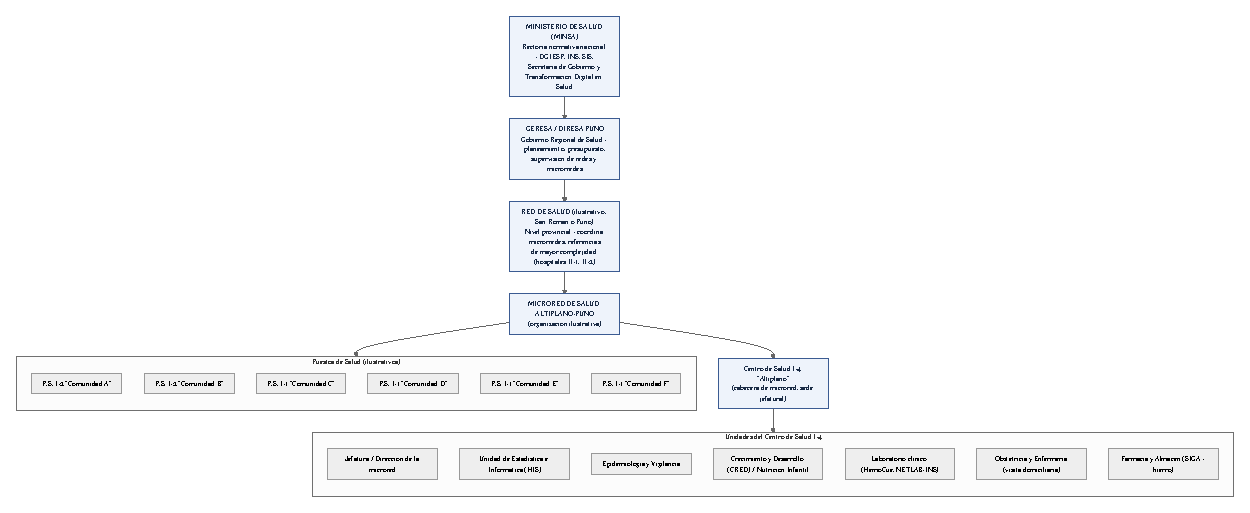
\includegraphics[width=0.8\linewidth,height=0.86\textheight,keepaspectratio]{assets/01-diagnostico/diagrama-01-estructura-organizacional.pdf}
\caption*{Diagrama 1 --- Estructura organizacional jerárquica de la Microred de Salud Altiplano-Puno (ilustrativa)}
\end{figure}

En este esquema, el Centro de Salud I-4 actúa como cabecera de red, concentrando las capacidades resolutivas más altas (laboratorio, mayor disponibilidad de personal profesional) y ejerciendo funciones de coordinación administrativa y de sistemas de información sobre los puestos de salud I-1/I-2 de las comunidades circundantes, que suelen operar con personal técnico o de enfermería en solitario, mayor dependencia de brigadas itinerantes y mayor exposición a discontinuidad de servicios básicos (electricidad, conectividad). La Jefatura de la microred reporta funcionalmente a la Red de Salud provincial y esta, a su vez, a la GERESA/DIRESA Puno, en un esquema donde las decisiones presupuestales relevantes (compra de equipos, ampliación de plazas) suelen requerir aprobación en niveles superiores, lo que introduce fricción y tiempos de respuesta prolongados para la adopción de innovaciones tecnológicas en el nivel operativo.

Adicionalmente, la microred se articula horizontalmente con actores de gobierno local (municipalidades distritales y provinciales, con competencias en saneamiento y programas sociales) y con programas sociales intersectoriales (Qali Warma, Cuna Más, Juntos), cuya coordinación es generalmente informal y no está soportada por sistemas de información compartidos, dependiendo de reuniones periódicas y comunicación telefónica o por mensajería instantánea.

\subsubsection{1.1.3 Cadena de valor}\label{cadena-de-valor}

Adaptando el modelo de cadena de valor de Porter al proceso asistencial de tamizaje y manejo de la anemia infantil, se identifican las siguientes actividades primarias y de apoyo en la Microred de Salud Altiplano-Puno:

\begin{figure}[H]
\centering
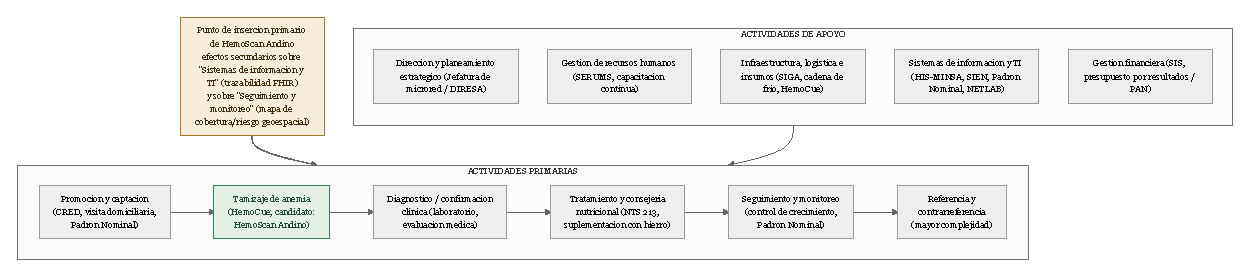
\includegraphics[width=0.95\linewidth,height=0.86\textheight,keepaspectratio]{assets/01-diagnostico/diagrama-02-cadena-valor.pdf}
\caption*{Diagrama 2 --- Cadena de valor del proceso de tamizaje y atención de la anemia infantil}
\end{figure}

HemoScan Andino se inserta principalmente en la actividad primaria de \textbf{tamizaje}, ofreciendo una alternativa no invasiva a la punción capilar, pero su valor se extiende horizontalmente hacia dos actividades de apoyo: primero, hacia los \textbf{sistemas de información y TI}, al generar recursos FHIR (Observation, Provenance, AuditEvent, Consent, Device, Patient) que pueden alimentar el HIS-MINSA y el Padrón Nominal de manera estructurada, reduciendo el subregistro; y segundo, de manera indirecta, hacia el \textbf{seguimiento y monitoreo poblacional}, al proveer datos agregados y anonimizados que permiten construir mapas de cobertura y riesgo geoespacial (mediante MapLibre GL JS, PMTiles y H3) útiles para la priorización de recursos por parte de la Jefatura de microred y la DIRESA. Es importante subrayar que el sistema \textbf{no reemplaza} la actividad de ``Diagnóstico/Confirmación clínica'': su función es de tamizaje que deriva a confirmación, preservando el rol del personal de salud como responsable final de la decisión clínica, en línea con el principio de supervisión humana exigido por el DS 115-2025-PCM para sistemas de inteligencia artificial en sectores de alto riesgo como salud.

\subsubsection{1.1.4 Mapa de stakeholders}\label{mapa-de-stakeholders}

Se identifican catorce grupos de interés relevantes para el ecosistema de la Microred de Salud Altiplano-Puno y, por extensión, para la viabilidad de HemoScan Andino. La clasificación de influencia e interés sigue una lógica cualitativa tipo matriz de Mendelow (alto/medio/bajo).

{\small
\begin{longtable}[]{@{}
  >{\raggedright\arraybackslash}p{(\linewidth - 10\tabcolsep) * \real{0.1667}}
  >{\raggedright\arraybackslash}p{(\linewidth - 10\tabcolsep) * \real{0.1667}}
  >{\raggedright\arraybackslash}p{(\linewidth - 10\tabcolsep) * \real{0.1667}}
  >{\raggedright\arraybackslash}p{(\linewidth - 10\tabcolsep) * \real{0.1667}}
  >{\raggedright\arraybackslash}p{(\linewidth - 10\tabcolsep) * \real{0.1667}}
  >{\raggedright\arraybackslash}p{(\linewidth - 10\tabcolsep) * \real{0.1667}}@{}}
\toprule\noalign{}
\begin{minipage}[b]{\linewidth}\raggedright
Stakeholder
\end{minipage} & \begin{minipage}[b]{\linewidth}\raggedright
Tipo
\end{minipage} & \begin{minipage}[b]{\linewidth}\raggedright
Interés / expectativa principal
\end{minipage} & \begin{minipage}[b]{\linewidth}\raggedright
Influencia
\end{minipage} & \begin{minipage}[b]{\linewidth}\raggedright
Interés
\end{minipage} & \begin{minipage}[b]{\linewidth}\raggedright
Estrategia de relacionamiento
\end{minipage} \\
\midrule\noalign{}
\endhead
\bottomrule\noalign{}
\endlastfoot
Niños menores de 3 años (beneficiarios finales) & Externo primario & Detección temprana y tratamiento oportuno de anemia, sin dolor ni trauma & Bajo (no decide directamente) & Alto (afectado directo) & Proteger: diseño centrado en no invasividad y consentimiento informado de tutores \\
Madres, padres y cuidadores & Externo primario & Confianza en el método, rapidez, resultados comprensibles, consejería útil & Medio-Alto (deciden participación) & Alto & Involucrar activamente: comunicación clara, pertinencia intercultural, consentimiento (Ley 29733) \\
Personal de salud de la microred (médicos, obstetras, enfermeras, técnicos) & Interno & Herramienta que reduzca carga operativa, fácil de usar, no aumente riesgo legal & Alto (usuarios operativos y prescriptores de confianza clínica) & Alto & Gestionar de cerca: capacitación, participación en el diseño, retroalimentación continua \\
Jefatura de la Microred / Red de Salud & Interno-gestor & Mejora de indicadores, cumplimiento de metas DIRESA, gestión eficiente de recursos & Alto & Alto & Gestionar de cerca: aliado clave para piloto y adopción institucional \\
GERESA / DIRESA Puno & Externo --- decisor de política y presupuesto & Reducción de indicadores regionales de anemia, cumplimiento normativo, viabilidad presupuestal & Muy alto & Alto & Gestionar de cerca: cliente potencial B2G, requiere validación formal y convenio \\
Municipalidades distritales / provinciales & Externo --- potencial cofinanciador & Mejora de indicadores locales de salud infantil, visibilidad política & Medio-Alto & Medio & Mantener informado: potencial fuente de cofinanciamiento en Fase 1 \\
MINSA (nivel central: DGIESP, Secretaría de Gobierno y Transformación Digital) & Externo --- normativo & Cumplimiento de NTS 213-MINSA/DGIESP-2024, interoperabilidad nacional (REUNIS, HIS) & Alto & Medio & Mantener informado: interlocutor para escalamiento e interoperabilidad nacional \\
RENIEC / MEF (Padrón Nominal) & Externo --- socio de datos & Calidad e integridad del registro nominal de niños para programas sociales & Medio & Medio & Mantener informado: interoperabilidad técnica de identificación de beneficiarios \\
Comité de Ética en Investigación (por constituir) & Externo --- regulador de la validación & Protección de derechos de los menores, rigor metodológico del estudio & Alto (bloqueante si no se constituye) & Alto & Gestionar de cerca: \textbf{requisito previo obligatorio} antes de trabajo de campo \\
Universidad Peruana Unión (UPeU) & Interno --- aliado académico & Validación científica, cumplimiento de estándares de tesis, prestigio institucional & Alto & Alto & Gestionar de cerca: asesoría metodológica y respaldo institucional \\
Equipo HemoScan Andino (futura HemoScan Andino S.A.C.) & Interno --- proveedor/emprendedor & Validar la solución, generar tracción para Fase 1, constituir la empresa & Alto & Alto & Motor del proyecto: gestión directa \\
Cooperación internacional / ONGs de nutrición infantil & Externo --- potencial financiador & Impacto medible en indicadores de anemia y desnutrición crónica infantil & Medio & Medio-Alto & Mantener informado: fuente de financiamiento no gubernamental para Fase 1 \\
Autoridad Nacional de Protección de Datos Personales & Externo --- regulador legal & Cumplimiento de la Ley N.° 29733 en el tratamiento de datos de salud de menores & Alto & Bajo-Medio & Satisfacer: cumplimiento normativo proactivo, no solo reactivo \\
Proveedores de componentes electrónicos (AS7341, MAX30102, ESP32-S3) & Externo --- cadena de suministro & Continuidad comercial, volumen de compra & Bajo & Bajo & Monitorear: gestionar riesgo de disponibilidad y sustitución de componentes \\
\end{longtable}
}

La lectura estratégica de este mapa evidencia que los actores de \textbf{mayor influencia y mayor interés} ---GERESA/DIRESA Puno, la Jefatura de la microred, el personal de salud y el Comité de Ética por constituir--- deben concentrar el esfuerzo de relacionamiento institucional del equipo HemoScan Andino en la fase de validación (Fase 0), dado que sin su involucramiento activo no es posible avanzar hacia el piloto pagado (Fase 1). En contraste, actores como la cooperación internacional o los proveedores de hardware, si bien relevantes, pueden gestionarse con una cadencia de comunicación menos intensiva en esta etapa inicial.

\begin{center}\rule{0.5\linewidth}{0.5pt}\end{center}

\subsection{1.2 Análisis Estratégico}\label{anuxe1lisis-estratuxe9gico}

\subsubsection{1.2.1 Misión, visión y objetivos estratégicos}\label{misiuxf3n-visiuxf3n-y-objetivos-estratuxe9gicos}

Dado que la Microred de Salud Altiplano-Puno es una organización ilustrativa, la misión y visión aquí formuladas constituyen una \textbf{construcción referencial} elaborada por el equipo de tesis, alineada a los lineamientos genéricos del sector salud peruano (Ley General de Salud, Plan Nacional Concertado de Salud, orientaciones sectoriales de reducción de anemia y desnutrición crónica infantil) y a la lógica institucional típica de un Proyecto Educativo Institucional (PEI) de una microred de primer nivel de atención. Estas declaraciones deberán contrastarse con los documentos de gestión oficiales (PEI, Reglamento de Organización y Funciones) de la microred real que eventualmente participe en el proyecto.

\textbf{Misión (referencial):} ``Brindar servicios de salud integral, con enfoque preventivo-promocional e intercultural, a la población de su jurisdicción altoandina, priorizando la reducción de la anemia y la desnutrición crónica infantil, mediante personal competente, gestión eficiente de recursos y articulación intersectorial permanente.''

\textbf{Visión (referencial):} ``Ser reconocida, hacia el final de la década, como una red de establecimientos de primer nivel de atención de referencia en la región Puno por la calidad, oportunidad y enfoque preventivo de su atención materno-infantil, incorporando de manera responsable innovaciones tecnológicas al servicio de la reducción de las brechas de salud altoandinas.''

\textbf{Objetivos estratégicos (referenciales, alineados a las prioridades sectoriales de lucha contra la anemia y la desnutrición crónica infantil y al marco de la NTS 213-MINSA/DGIESP-2024):}

{\small
\begin{longtable}[]{@{}
  >{\raggedright\arraybackslash}p{(\linewidth - 2\tabcolsep) * \real{0.5000}}
  >{\raggedright\arraybackslash}p{(\linewidth - 2\tabcolsep) * \real{0.5000}}@{}}
\toprule\noalign{}
\begin{minipage}[b]{\linewidth}\raggedright
Código
\end{minipage} & \begin{minipage}[b]{\linewidth}\raggedright
Objetivo estratégico
\end{minipage} \\
\midrule\noalign{}
\endhead
\bottomrule\noalign{}
\endlastfoot
OE1 & Reducir la prevalencia de anemia y desnutrición crónica infantil en la jurisdicción de la microred. \\
OE2 & Fortalecer la capacidad resolutiva y de tamizaje temprano de los establecimientos de primer nivel de atención. \\
OE3 & Mejorar la calidad, oportunidad e interoperabilidad del sistema de información en salud materno-infantil. \\
OE4 & Fortalecer la articulación intersectorial e intergubernamental (municipios, programas sociales, Padrón Nominal). \\
OE5 & Garantizar la pertinencia intercultural, la protección de datos personales y la satisfacción del usuario en la prestación del servicio. \\
\end{longtable}
}

Estos cinco objetivos constituyen el eje de referencia frente al cual se contrastarán, más adelante (sección 1.2.5), las brechas estratégicas detectadas en el diagnóstico digital.

\subsubsection{1.2.2 Análisis FODA}\label{anuxe1lisis-foda}

El análisis FODA se construyó a partir de la revisión de la literatura citada en el proyecto (ENDES 2025; Gonzales et al., 2025; Baquerizo-Sedano et al., 2025), del marco normativo aplicable (NTS 213-MINSA/DGIESP-2024; DS 115-2025-PCM; Ley N.° 29733) y del conocimiento general, documentado públicamente, sobre las condiciones operativas de los establecimientos de salud de primer nivel en zonas rurales altoandinas del Perú. Cada factor incluye una columna de sustento para reforzar su carácter fundamentado y no meramente enunciativo.

\textbf{Fortalezas (internas)}

{\small
\begin{longtable}[]{@{}
  >{\raggedright\arraybackslash}p{(\linewidth - 4\tabcolsep) * \real{0.3333}}
  >{\raggedright\arraybackslash}p{(\linewidth - 4\tabcolsep) * \real{0.3333}}
  >{\raggedright\arraybackslash}p{(\linewidth - 4\tabcolsep) * \real{0.3333}}@{}}
\toprule\noalign{}
\begin{minipage}[b]{\linewidth}\raggedright
N.°
\end{minipage} & \begin{minipage}[b]{\linewidth}\raggedright
Fortaleza
\end{minipage} & \begin{minipage}[b]{\linewidth}\raggedright
Sustento / evidencia
\end{minipage} \\
\midrule\noalign{}
\endhead
\bottomrule\noalign{}
\endlastfoot
F1 & Presencia física de establecimientos de primer nivel en zonas rurales dispersas, con vínculo comunitario ya establecido & Estructura típica de microrredes rurales del sector (Centro de Salud cabecera + puestos de salud satélite descrita en 1.1.2) \\
F2 & Experiencia previa del personal en el uso del método de referencia HemoCue y en protocolos CRED & Práctica clínica estándar del primer nivel de atención bajo la NTS 213-MINSA/DGIESP-2024 \\
F3 & Vínculo operativo ya existente con el Padrón Nominal y programas sociales (Qali Warma, Cuna Más, Juntos) & Articulación intersectorial constitutiva del modelo MINSA-MEF-RENIEC del Padrón Nominal \\
F4 & Uso extendido de teléfonos móviles por parte del personal de salud, aun de forma informal & Práctica documentada de uso de mensajería instantánea para coordinación operativa en establecimientos rurales \\
F5 & Alineación con una prioridad de política pública de alto perfil (lucha contra la anemia infantil) & Prevalencia regional de 56.1 \% en menores de 3 años (ENDES 2025), la más alta del país \\
\end{longtable}
}

\textbf{Debilidades (internas)}

{\small
\begin{longtable}[]{@{}
  >{\raggedright\arraybackslash}p{(\linewidth - 4\tabcolsep) * \real{0.3333}}
  >{\raggedright\arraybackslash}p{(\linewidth - 4\tabcolsep) * \real{0.3333}}
  >{\raggedright\arraybackslash}p{(\linewidth - 4\tabcolsep) * \real{0.3333}}@{}}
\toprule\noalign{}
\begin{minipage}[b]{\linewidth}\raggedright
N.°
\end{minipage} & \begin{minipage}[b]{\linewidth}\raggedright
Debilidad
\end{minipage} & \begin{minipage}[b]{\linewidth}\raggedright
Sustento / evidencia
\end{minipage} \\
\midrule\noalign{}
\endhead
\bottomrule\noalign{}
\endlastfoot
D1 & Quiebres de stock recurrentes de insumos HemoCue (microcuvetas, lancetas) & Dependencia de insumos importados fungibles en cadena logística rural extensa \\
D2 & Conectividad a internet y suministro eléctrico intermitentes en puestos de salud rurales & Condición estructural de zonas altoandinas dispersas (sección 1.1.1) \\
D3 & Alta rotación de personal por el régimen SERUMS, con discontinuidad en la capacitación & Régimen de Servicio Rural y Urbano Marginal de Salud (SERUMS), de duración anual, aplicable a establecimientos de primer nivel \\
D4 & Sistemas de información fragmentados y no interoperables entre sí (HIS, SIEN, Padrón Nominal) & Detallado en el diagnóstico digital, sección 1.3.1 \\
D5 & Ausencia de una capa de corrección de hemoglobina por altitud auditable y estandarizada & Riesgo de sobre/subdiagnóstico documentado por Gonzales et al.~(2025) y Baquerizo-Sedano et al.~(2025) \\
D6 & Bajo nivel de gobierno de datos y de ciberseguridad para datos sensibles de salud de menores & Ausencia de controles verificados frente a las exigencias de la Ley N.° 29733 \\
D7 & Dependencia del método invasivo HemoCue como única alternativa de tamizaje disponible & Estructura de la cadena de valor descrita en 1.1.3; no se identifican alternativas no invasivas desplegadas \\
\end{longtable}
}

\textbf{Oportunidades (externas)}

{\small
\begin{longtable}[]{@{}
  >{\raggedright\arraybackslash}p{(\linewidth - 4\tabcolsep) * \real{0.3333}}
  >{\raggedright\arraybackslash}p{(\linewidth - 4\tabcolsep) * \real{0.3333}}
  >{\raggedright\arraybackslash}p{(\linewidth - 4\tabcolsep) * \real{0.3333}}@{}}
\toprule\noalign{}
\begin{minipage}[b]{\linewidth}\raggedright
N.°
\end{minipage} & \begin{minipage}[b]{\linewidth}\raggedright
Oportunidad
\end{minipage} & \begin{minipage}[b]{\linewidth}\raggedright
Sustento / evidencia
\end{minipage} \\
\midrule\noalign{}
\endhead
\bottomrule\noalign{}
\endlastfoot
O1 & Marco normativo que exige explícitamente mejorar el tamizaje y la consejería nutricional de anemia & NTS 213-MINSA/DGIESP-2024 \\
O2 & Priorización nacional y regional histórica de la lucha contra la anemia y la desnutrición infantil & Política sectorial multianual de reducción de anemia y desnutrición crónica infantil \\
O3 & Marco regulatorio de IA en salud que, aunque exigente, habilita el uso de IA auditable con supervisión humana & DS 115-2025-PCM (reglamento de la Ley 31814), salud como sector de alto riesgo \\
O4 & Disponibilidad creciente de fondos de cooperación internacional para innovación en salud rural materno-infantil & Tendencia documentada de financiamiento de cooperación internacional en salud materno-infantil andina \\
O5 & Penetración creciente de teléfonos inteligentes y módulos Bluetooth Low Energy de bajo costo, incluso en zonas rurales & Tendencia tecnológica de abaratamiento de componentes IoT (ESP32, BLE) \\
O6 & Posibilidad de alianza formal con la Universidad Peruana Unión para investigación y validación científica & Naturaleza de tesis universitaria del proyecto (UPeU, Ingeniería de Sistemas, sede Juliaca) \\
\end{longtable}
}

\textbf{Amenazas (externas)}

{\small
\begin{longtable}[]{@{}
  >{\raggedright\arraybackslash}p{(\linewidth - 4\tabcolsep) * \real{0.3333}}
  >{\raggedright\arraybackslash}p{(\linewidth - 4\tabcolsep) * \real{0.3333}}
  >{\raggedright\arraybackslash}p{(\linewidth - 4\tabcolsep) * \real{0.3333}}@{}}
\toprule\noalign{}
\begin{minipage}[b]{\linewidth}\raggedright
N.°
\end{minipage} & \begin{minipage}[b]{\linewidth}\raggedright
Amenaza
\end{minipage} & \begin{minipage}[b]{\linewidth}\raggedright
Sustento / evidencia
\end{minipage} \\
\midrule\noalign{}
\endhead
\bottomrule\noalign{}
\endlastfoot
A1 & Alta dispersión geográfica y difícil accesibilidad vial, que encarece la logística de cualquier solución, incluida HemoScan & Condición estructural altoandina descrita en 1.1.1 \\
A2 & Restricciones presupuestales del sector público y cambios de prioridad tras ciclos electorales regionales/municipales & Dependencia de presupuesto público de gobiernos regionales (modelo B2G) \\
A3 & Resistencia al cambio y eventual desconfianza de la población hacia tecnologías médicas no familiares & Riesgo típico de adopción tecnológica en salud comunitaria intercultural \\
A4 & Exigencias de protección de datos personales de menores que, de no gestionarse bien, pueden ralentizar la adopción & Ley N.° 29733, sensibilidad máxima por tratarse de datos de salud de menores de edad \\
A5 & Riesgo de que una calibración por altitud mal validada derive en sobre/subdiagnóstico y erosione la confianza institucional & Advertencia explícita de Gonzales et al.~(2025) y Baquerizo-Sedano et al.~(2025) sobre el efecto de la altitud en la interpretación de hemoglobina \\
A6 & Posible entrada de soluciones competidoras de bajo costo, dado que la barrera de entrada de hardware no es muy alta & Análisis de entorno competitivo, sección 1.1.1 \\
\end{longtable}
}

Del cruce cualitativo de estos factores se desprende que la principal tensión estratégica de la organización ilustrativa ---y, por extensión, del proyecto HemoScan Andino--- es la existencia de una oportunidad de política pública clara y urgente (O1, O2, F5) confrontada con debilidades tecnológicas profundas (D4, D5, D6) y amenazas regulatorias/de confianza no triviales (A4, A5). Esta tensión se desarrolla con mayor detalle en la matriz FODA cruzada del Anexo E.

\subsubsection{1.2.3 Análisis PESTEL}\label{anuxe1lisis-pestel}

Aunque el formato de la rúbrica considera el análisis PESTEL opcional según la complejidad del proyecto, se incluye en este diagnóstico de manera obligatoria dado que HemoScan Andino opera en la intersección de al menos tres marcos regulatorios de alta complejidad (normativa técnica de salud, reglamento de inteligencia artificial y ley de protección de datos personales de menores), además de un factor ambiental (altitud) que es, a la vez, condición fisiológica del problema clínico y condición de diseño del hardware.

{\small
\begin{longtable}[]{@{}
  >{\raggedright\arraybackslash}p{(\linewidth - 4\tabcolsep) * \real{0.3333}}
  >{\raggedright\arraybackslash}p{(\linewidth - 4\tabcolsep) * \real{0.3333}}
  >{\raggedright\arraybackslash}p{(\linewidth - 4\tabcolsep) * \real{0.3333}}@{}}
\toprule\noalign{}
\begin{minipage}[b]{\linewidth}\raggedright
Factor
\end{minipage} & \begin{minipage}[b]{\linewidth}\raggedright
Descripción
\end{minipage} & \begin{minipage}[b]{\linewidth}\raggedright
Implicancia para la Microred / HemoScan Andino
\end{minipage} \\
\midrule\noalign{}
\endhead
\bottomrule\noalign{}
\endlastfoot
\textbf{Político} & Existencia de una política sectorial de priorización de la lucha contra la anemia y la desnutrición crónica infantil, con posibles cambios de autoridades en GERESA/DIRESA y municipios tras procesos electorales regionales & Ventana de oportunidad para posicionar el proyecto como alineado a metas de gestión, pero con riesgo de discontinuidad de patrocinio institucional ante cambios de gestión \\
\textbf{Económico} & Restricciones presupuestales estructurales de los gobiernos regionales y dependencia de transferencias del MEF (canon, FONCOMUN); altos costos logísticos de operación en zona altoandina dispersa & El modelo B2G de HemoScan Andino debe diseñarse con estructuras de costo flexibles (venta/alquiler) y demostrar retorno medible para justificar la inversión pública \\
\textbf{Social} & Prevalencia de anemia infantil de 56.1 \% en menores de 3 años (ENDES 2025); diversidad lingüística quechua/aymara; dispersión poblacional; percepción cultural de la punción capilar como procedimiento doloroso y de rechazo, especialmente en tamizajes repetidos & Exige diseño de interfaz y consejería con pertinencia intercultural, y valida la propuesta de valor de la no invasividad como palanca de aceptación social \\
\textbf{Tecnológico} & Conectividad a internet y suministro eléctrico intermitentes; creciente disponibilidad de smartphones de gama media y módulos BLE de bajo costo; avances en inferencia embebida (TinyML, ONNX/TFLite) que habilitan procesamiento offline & Justifica y valida técnicamente la arquitectura offline-first de HemoScan Andino como respuesta directa a la brecha de conectividad rural \\
\textbf{Ecológico / ambiental} & Altitud extrema (referencial 3,800 m s. n.~m.) con efecto fisiológico sobre la hemoglobina; clima frígido y variable que exige hardware robusto (batería, sellado, tolerancia térmica); radiación solar intensa & Fundamenta la necesidad central de la capa de autocalibración por altitud (GPS + Modelo Digital de Elevación) y condiciona los requisitos no funcionales de diseño de hardware del nodo ESP32-S3 \\
\textbf{Legal} & Ley N.° 29733 (protección de datos personales, máxima sensibilidad por tratarse de datos de salud de menores de edad); DS 115-2025-PCM (reglamento de IA de la Ley 31814, salud como sector de alto riesgo que exige supervisión humana y trazabilidad); NTS 213-MINSA/DGIESP-2024 (manejo de anemia); eventual necesidad futura de registro sanitario del dispositivo & Impone requisitos de diseño obligatorios: consentimiento informado explícito, trazabilidad FHIR auditable (Provenance, AuditEvent, Consent), y arquitectura de tamizaje que derive a confirmación clínica sin decisión autónoma de IA \\
\end{longtable}
}

El análisis PESTEL confirma que el factor \textbf{legal} y el factor \textbf{ecológico/ambiental} son, para este proyecto en particular, más determinantes de lo habitual: no se trata de riesgos periféricos, sino de restricciones de diseño que están en el núcleo mismo de la propuesta de valor (la corrección por altitud) y de su licencia social y regulatoria para operar (la protección de datos de menores y la supervisión humana exigida por ley).

\subsubsection{1.2.4 Factores críticos de éxito}\label{factores-cruxedticos-de-uxe9xito}

A partir del análisis estratégico precedente, se identifican cinco factores críticos de éxito (FCE) para que la intervención de HemoScan Andino sobre la Microred de Salud Altiplano-Puno ---y, por extensión, sobre cualquier microred real que eventualmente participe--- logre sus objetivos:

\begin{enumerate}
\def\labelenumi{\arabic{enumi}.}
\tightlist
\item
  \textbf{Validación clínica robusta de la corrección por altitud.} Sin evidencia sólida de que el algoritmo de autocalibración reduce, y no aumenta, el riesgo de sobre/subdiagnóstico frente al método de referencia, el proyecto carece de legitimidad clínica (Gonzales et al., 2025; Baquerizo-Sedano et al., 2025).
\item
  \textbf{Interoperabilidad real, no solo declarada, con el HIS-MINSA y el Padrón Nominal.} La generación de recursos FHIR debe traducirse en integración efectiva con los sistemas oficiales, o el proyecto reproducirá la fragmentación de información ya diagnosticada (sección 1.3).
\item
  \textbf{Operación confiable en modo offline-first.} Dada la intermitencia de conectividad y energía eléctrica en los puestos de salud rurales, la arquitectura debe garantizar funcionalidad plena sin conexión permanente.
\item
  \textbf{Adopción y apropiación por parte del personal de salud.} La facilidad de uso, la capacitación adecuada y la percepción de utilidad (reducción de carga operativa, no aumento de esta) son determinantes para la sostenibilidad del uso más allá del piloto.
\item
  \textbf{Cumplimiento normativo integral y proactivo.} El cumplimiento simultáneo de la NTS 213-MINSA/DGIESP-2024, el DS 115-2025-PCM y la Ley N.° 29733 no es opcional ni puede abordarse de manera reactiva, dado que cualquier incumplimiento compromete la viabilidad legal y ética del proyecto, especialmente al tratarse de datos de menores de edad.
\end{enumerate}

A estos cinco se añade un factor condicionante, no estrictamente de éxito del producto sino de viabilidad metodológica: \textbf{la formalización de un convenio institucional con una microred real y la constitución de un comité de ética en investigación}, sin los cuales ninguno de los cinco FCE anteriores puede validarse empíricamente.

\subsubsection{1.2.5 Síntesis de brechas estratégicas identificadas}\label{suxedntesis-de-brechas-estratuxe9gicas-identificadas}

Con el fin de reforzar la trazabilidad entre los objetivos estratégicos formulados en 1.2.1 y los hallazgos de este diagnóstico, se presenta la siguiente matriz de síntesis:

{\small
\begin{longtable}[]{@{}
  >{\raggedright\arraybackslash}p{(\linewidth - 6\tabcolsep) * \real{0.2500}}
  >{\raggedright\arraybackslash}p{(\linewidth - 6\tabcolsep) * \real{0.2500}}
  >{\raggedright\arraybackslash}p{(\linewidth - 6\tabcolsep) * \real{0.2500}}
  >{\raggedright\arraybackslash}p{(\linewidth - 6\tabcolsep) * \real{0.2500}}@{}}
\toprule\noalign{}
\begin{minipage}[b]{\linewidth}\raggedright
Objetivo estratégico
\end{minipage} & \begin{minipage}[b]{\linewidth}\raggedright
Situación actual (diagnóstico)
\end{minipage} & \begin{minipage}[b]{\linewidth}\raggedright
Brecha identificada
\end{minipage} & \begin{minipage}[b]{\linewidth}\raggedright
Evidencia / sustento
\end{minipage} \\
\midrule\noalign{}
\endhead
\bottomrule\noalign{}
\endlastfoot
OE1 --- Reducir anemia y desnutrición infantil & Prevalencia de 56.1 \% en menores de 3 años, la más alta del país; tamizaje dependiente de un único método invasivo & Brecha de cobertura y de precisión diagnóstica ajustada a altitud & ENDES 2025; Gonzales et al.~(2025); Baquerizo-Sedano et al.~(2025) \\
OE2 --- Fortalecer capacidad resolutiva de tamizaje & HemoCue como única alternativa, con quiebres de stock e insumos limitados & Brecha de disponibilidad tecnológica no invasiva y de continuidad de insumos & Sección 1.1.1 y Debilidad D1, D7 \\
OE3 --- Mejorar sistema de información en salud & HIS, SIEN y Padrón Nominal operan de forma fragmentada, sin interoperabilidad plena & Brecha de interoperabilidad y trazabilidad digital & Sección 1.3.1 y Debilidad D4 \\
OE4 --- Fortalecer articulación intersectorial & Coordinación con municipios y programas sociales mayormente informal, sin sistemas compartidos & Brecha de gobernanza de datos intersectorial & Sección 1.1.2 y 1.3.3 \\
OE5 --- Pertinencia intercultural y protección de datos & Bajo nivel de gobierno de datos frente a exigencias de la Ley 29733; ausencia de mecanismos de consentimiento digital auditable & Brecha de cumplimiento normativo y de gestión de confianza comunitaria & Debilidad D6; Amenaza A3, A4; DS 115-2025-PCM \\
\end{longtable}
}

Esta síntesis constituye el puente directo entre el diagnóstico estratégico (1.2) y el diagnóstico digital/TI (1.3) que se desarrolla a continuación, y será retomada en la sección 1.4 para fundamentar la justificación de la intervención.

\begin{center}\rule{0.5\linewidth}{0.5pt}\end{center}

\subsection{1.3 Diagnóstico Digital / TI}\label{diagnuxf3stico-digital-ti}

\subsubsection{1.3.1 Inventario de sistemas de información existentes}\label{inventario-de-sistemas-de-informaciuxf3n-existentes}

Una microred de salud de primer nivel de atención en el Perú interactúa típicamente con un conjunto de sistemas de información nacionales, cuya coexistencia no siempre implica interoperabilidad real entre sí. El siguiente inventario recoge los sistemas relevantes para el proceso de tamizaje y seguimiento de anemia infantil:

{\small
\begin{longtable}[]{@{}
  >{\raggedright\arraybackslash}p{(\linewidth - 8\tabcolsep) * \real{0.2000}}
  >{\raggedright\arraybackslash}p{(\linewidth - 8\tabcolsep) * \real{0.2000}}
  >{\raggedright\arraybackslash}p{(\linewidth - 8\tabcolsep) * \real{0.2000}}
  >{\raggedright\arraybackslash}p{(\linewidth - 8\tabcolsep) * \real{0.2000}}
  >{\raggedright\arraybackslash}p{(\linewidth - 8\tabcolsep) * \real{0.2000}}@{}}
\toprule\noalign{}
\begin{minipage}[b]{\linewidth}\raggedright
Sistema
\end{minipage} & \begin{minipage}[b]{\linewidth}\raggedright
Entidad responsable
\end{minipage} & \begin{minipage}[b]{\linewidth}\raggedright
Función principal
\end{minipage} & \begin{minipage}[b]{\linewidth}\raggedright
Nivel de integración/interoperabilidad
\end{minipage} & \begin{minipage}[b]{\linewidth}\raggedright
Limitación principal
\end{minipage} \\
\midrule\noalign{}
\endhead
\bottomrule\noalign{}
\endlastfoot
HIS-MINSA (Sistema de Información de Hospitales / Aplicativo HIS) & MINSA & Registro de atenciones y prestaciones de salud a nivel de establecimiento & Medio (reporta a nivel central, pero con baja integración horizontal con otros sistemas) & Registro mayormente retrospectivo, dependiente de digitación manual posterior a la atención \\
SIS (Seguro Integral de Salud) & MINSA / SIS & Afiliación y financiamiento de prestaciones de la población sin seguro & Bajo-Medio con sistemas clínicos & Orientado a facturación/financiamiento, no a seguimiento clínico longitudinal \\
SIEN (Sistema de Información del Estado Nutricional) & MINSA / INS & Registro de indicadores antropométricos y estado nutricional infantil & Bajo con HIS y Padrón Nominal & Alimentado con retraso; no integra variables de hemoglobina ajustadas por altitud de forma estandarizada \\
Padrón Nominal & MINSA -- MEF -- RENIEC & Registro nominal de niñas y niños menores de 6 años para seguimiento de programas sociales y de salud & Medio (fuente de identificación de beneficiarios entre sectores) & Actualización dependiente de reportes periódicos de los establecimientos, con rezagos \\
NETLAB & Instituto Nacional de Salud (INS) & Reporte de resultados de laboratorio de la red de salud pública & Bajo en establecimientos rurales de primer nivel & Uso limitado en puestos de salud sin laboratorio propio o sin conectividad estable \\
REUNIS (Repositorio Único Nacional de Información en Salud) & MINSA & Repositorio nacional de información en salud para toma de decisiones & Bajo a nivel de microred (más orientado a consumo agregado nacional/regional) & Baja visibilidad y uso operativo directo en el nivel de establecimiento \\
SIGA (Sistema Integrado de Gestión Administrativa) & MEF / MINSA & Gestión logística y de almacenes (incluye insumos como microcuvetas HemoCue) & Medio & No está diseñado para predicción de quiebres de stock ni para priorización basada en riesgo epidemiológico \\
Registro manual de HemoCue (cuadernos/Excel) & Establecimiento de salud & Registro local de resultados de tamizaje de hemoglobina & Nulo (no digital, no auditable) & Alto riesgo de error de digitación, pérdida de información y ausencia de trazabilidad \\
Historia clínica & Establecimiento de salud & Registro clínico individual del paciente & Bajo (predominantemente física/en papel en zonas rurales; Historia Clínica Electrónica incipiente) & Fragmentación del expediente clínico y dificultad de seguimiento longitudinal \\
Mensajería instantánea informal (uso de ``shadow IT'') & Personal de salud (uso no oficial) & Coordinación operativa entre puestos de salud y cabecera de microred & No aplica (canal no oficial) & Sin respaldo institucional, sin trazabilidad, con riesgo de fuga de información sensible \\
\end{longtable}
}

Este inventario evidencia un patrón recurrente en el sector: la existencia de múltiples sistemas verticales, cada uno diseñado para un propósito administrativo específico (financiamiento, nutrición, identificación, logística), sin una capa de interoperabilidad horizontal robusta que permita una vista longitudinal e integrada del niño tamizado. La ausencia de un sistema digital y auditable específico para el registro de hemoglobina ajustada por altitud es, en este inventario, la brecha más directamente relevante para HemoScan Andino.

\subsubsection{1.3.2 Nivel de madurez digital}\label{nivel-de-madurez-digital}

Para evaluar la madurez digital de la organización ilustrativa se emplea una escala ordinal de cinco niveles, de uso común en modelos de madurez de tipo CMMI adaptados a gestión de TI: \textbf{Nivel 1 (Inicial/Ad hoc)} --- procesos no estandarizados, dependientes de esfuerzo individual; \textbf{Nivel 2 (Repetible)} --- existen prácticas que se repiten, pero sin documentación ni estandarización formal; \textbf{Nivel 3 (Definido)} --- procesos documentados y estandarizados a nivel institucional; \textbf{Nivel 4 (Gestionado)} --- procesos medidos y controlados cuantitativamente; \textbf{Nivel 5 (Optimizado)} --- mejora continua basada en datos e innovación sistemática.

La siguiente evaluación constituye un \textbf{juicio profesional ilustrativo del equipo de tesis} para la organización representativa, no el resultado de un instrumento de evaluación formal aplicado a una microred real; deberá sustituirse por una evaluación real ---por ejemplo, mediante un instrumento de autodiagnóstico de gobierno digital--- una vez formalizado un convenio institucional. Por rigor metodológico, las seis dimensiones se puntúan con \textbf{valores puntuales únicos} (no con rangos), de manera consistente con la naturaleza ordinal de la escala de 5 niveles: en versiones preliminares de este documento, dos de las seis dimensiones (``Datos y analítica'' e ``Innovación'') se habían expresado como rangos (p.~ej. ``1-2'' o ``3-4''), lo que introducía una inconsistencia de escala. Dado que se trata en cualquier caso de un juicio ilustrativo y no de una medición instrumental, se optó por fijar el valor puntual más conservador en lugar de mantener el rango, dejando esta decisión explícita aquí en vez de aparentar una precisión numérica que el propio equipo no tiene.

{\small
\begin{longtable}[]{@{}
  >{\raggedright\arraybackslash}p{(\linewidth - 6\tabcolsep) * \real{0.2500}}
  >{\raggedright\arraybackslash}p{(\linewidth - 6\tabcolsep) * \real{0.2500}}
  >{\raggedright\arraybackslash}p{(\linewidth - 6\tabcolsep) * \real{0.2500}}
  >{\raggedright\arraybackslash}p{(\linewidth - 6\tabcolsep) * \real{0.2500}}@{}}
\toprule\noalign{}
\begin{minipage}[b]{\linewidth}\raggedright
Dimensión
\end{minipage} & \begin{minipage}[b]{\linewidth}\raggedright
Nivel actual (1-5)
\end{minipage} & \begin{minipage}[b]{\linewidth}\raggedright
Descripción del hallazgo
\end{minipage} & \begin{minipage}[b]{\linewidth}\raggedright
Nivel deseado (referencial)
\end{minipage} \\
\midrule\noalign{}
\endhead
\bottomrule\noalign{}
\endlastfoot
Infraestructura tecnológica (conectividad, energía, equipos) & 2 & Conectividad y suministro eléctrico intermitentes en puestos de salud rurales; equipamiento informático escaso y desactualizado, concentrado en la cabecera de microred & 3 \\
Sistemas de información (HIS, SIEN, Padrón Nominal, etc.) & 2 & Sistemas verticales operativos pero fragmentados, con bajo nivel de integración horizontal (sección 1.3.1) & 4 \\
Datos y analítica (calidad, gobierno de datos, uso para decisiones) & 1 & Registro predominantemente manual del tamizaje de hemoglobina; ausencia de analítica geoespacial o predictiva para priorización de recursos & 4 \\
Gobierno de TI y ciberseguridad & 1 & Ausencia de políticas formales de seguridad de la información y protección de datos verificables a nivel de microred & 3 \\
Capacidades digitales del personal de salud & 2 & Uso funcional de aplicativos básicos (HIS) y de mensajería instantánea informal; alta rotación (SERUMS) que dificulta la consolidación de competencias digitales & 3 \\
Innovación (uso de IA, analítica avanzada, interoperabilidad estándar tipo FHIR) & 1 & Nula adopción identificada de inteligencia artificial o estándares de interoperabilidad clínica (FHIR) a nivel de establecimiento & 4 \\
\end{longtable}
}

El promedio simple de estas seis dimensiones puntuales (2 + 2 + 1 + 1 + 2 + 1 = 9; 9/6) ubica a la organización ilustrativa en un nivel de madurez digital \textbf{1.5 sobre 5}, es decir, entre ``Inicial'' y ``Repetible'', lo cual es consistente con el diagnóstico generalizado ---documentado en diversos informes públicos sobre gobierno digital en el sector salud peruano--- de que los establecimientos de primer nivel de atención en zonas rurales altoandinas presentan rezagos digitales estructurales frente a establecimientos urbanos de mayor complejidad. Esta brecha de madurez es, simultáneamente, una limitación (dificulta la adopción de cualquier tecnología nueva) y una oportunidad (el espacio de mejora es amplio y la mejora incremental es más visible).

\subsubsection{1.3.3 Brechas tecnológicas}\label{brechas-tecnoluxf3gicas}

A partir del inventario de sistemas y la evaluación de madurez digital, se identifican las siguientes brechas tecnológicas específicas:

\begin{enumerate}
\def\labelenumi{\arabic{enumi}.}
\tightlist
\item
  Conectividad a internet y suministro eléctrico intermitentes en puestos de salud rurales, que limitan la operación de cualquier sistema dependiente de conexión permanente.
\item
  Ausencia de un método de tamizaje de hemoglobina no invasivo, lo que perpetúa la dependencia exclusiva del método invasivo HemoCue.
\item
  Ausencia de una capa de corrección de hemoglobina por altitud que sea transparente, auditable y basada en modelo digital de elevación (en lugar de altitud cruda de GPS o de fórmulas genéricas no contextualizadas).
\item
  Fragmentación e interoperabilidad limitada entre HIS, SIEN, Padrón Nominal y NETLAB, que impide una vista longitudinal integrada del niño tamizado.
\item
  Ausencia de Historia Clínica Electrónica unificada en los puestos de salud rurales.
\item
  Registro del tamizaje de hemoglobina predominantemente manual (cuadernos o Excel local), sin trazabilidad digital ni respaldo auditable.
\item
  Bajo nivel de gobierno de datos y de controles de ciberseguridad frente a las exigencias de la Ley N.° 29733 para datos de salud de menores de edad.
\item
  Ausencia de mecanismos digitales de consentimiento informado auditable (recurso FHIR Consent) en los procesos actuales de tamizaje.
\item
  Falta de trazabilidad de procedencia y auditoría de los resultados clínicos (equivalente a los recursos FHIR Provenance y AuditEvent).
\item
  Ausencia de analítica geoespacial (mapas de cobertura y riesgo) que permita priorizar recursos limitados según concentración de casos.
\item
  Ausencia de mecanismos de aprendizaje federado o reentrenamiento colaborativo entre postas, que hoy operan como silos de información aislados.
\item
  Bajo nivel de digitalización logística predictiva (SIGA no anticipa quiebres de stock de insumos HemoCue en función de demanda proyectada).
\item
  Brecha de competencias digitales del personal, agravada por la alta rotación asociada al régimen SERUMS.
\item
  Ausencia de autenticación robusta y control de acceso basado en roles (RBAC) para sistemas clínicos a nivel de microred.
\item
  Falta de marco de gobierno de IA a nivel de establecimiento que dé cumplimiento operativo al DS 115-2025-PCM (documentación de supervisión humana, registro de decisiones asistidas por IA).
\end{enumerate}

\subsubsection{1.3.4 Problemas operativos asociados a TI}\label{problemas-operativos-asociados-a-ti}

Estas brechas tecnológicas se traducen en problemas operativos concretos que afectan el día a día de la microred ilustrativa:

\begin{itemize}
\tightlist
\item
  \textbf{Duplicidad y carga de registro manual.} El personal de salud debe registrar la misma información del paciente en múltiples soportes (cuaderno de HemoCue, HIS, SIEN, Padrón Nominal), incrementando el tiempo administrativo en desmedro de la atención directa y elevando el riesgo de error de transcripción.
\item
  \textbf{Demoras en la consolidación de reportes agregados hacia la DIRESA.} La falta de interoperabilidad obliga a consolidaciones manuales periódicas, retrasando la disponibilidad de información para la toma de decisiones regionales.
\item
  \textbf{Incapacidad de priorización geográfica de recursos en tiempo casi real.} Sin analítica geoespacial, la asignación de brigadas itinerantes o de insumos entre puestos de salud se basa en criterios históricos o informales, y no en patrones de riesgo actualizados (por ejemplo, técnicas de autocorrelación espacial como Getis-Ord Gi* o LISA).
\item
  \textbf{Pérdida de continuidad institucional del conocimiento por alta rotación de personal.} La capacitación recibida por el personal saliente (régimen SERUMS) no siempre se transfiere de manera sistematizada al personal entrante, al no existir un sistema digital de gestión del conocimiento o de soporte a la decisión clínica.
\item
  \textbf{Riesgo de incumplimiento normativo silencioso.} La ausencia de mecanismos digitales de consentimiento y trazabilidad implica que, aunque el personal actúe de buena fe, la microred no puede demostrar de manera auditable el cumplimiento de la Ley N.° 29733 ni, en el futuro, del DS 115-2025-PCM si llegara a incorporar herramientas de IA sin la debida gobernanza.
\end{itemize}

\begin{center}\rule{0.5\linewidth}{0.5pt}\end{center}

\subsection{1.4 Identificación del Problema}\label{identificaciuxf3n-del-problema}

\subsubsection{1.4.1 Definición estructurada del problema}\label{definiciuxf3n-estructurada-del-problema}

\textbf{Problema central:} \emph{La Microred de Salud Altiplano-Puno (organización ilustrativa) carece de un sistema de tamizaje de anemia infantil que sea preciso en el contexto fisiológico de altitud, no invasivo, interoperable con los sistemas oficiales de información en salud y auditable en su trazabilidad, lo que contribuye a perpetuar un patrón de sub- y sobrediagnóstico, subregistro epidemiológico y bajo rendimiento (throughput) de tamizaje en la población menor de 3 años de su jurisdicción.}

Para efectos de precisión metodológica, este problema se estructura en los siguientes elementos:

{\small
\begin{longtable}[]{@{}
  >{\raggedright\arraybackslash}p{(\linewidth - 2\tabcolsep) * \real{0.5000}}
  >{\raggedright\arraybackslash}p{(\linewidth - 2\tabcolsep) * \real{0.5000}}@{}}
\toprule\noalign{}
\begin{minipage}[b]{\linewidth}\raggedright
Elemento
\end{minipage} & \begin{minipage}[b]{\linewidth}\raggedright
Descripción
\end{minipage} \\
\midrule\noalign{}
\endhead
\bottomrule\noalign{}
\endlastfoot
¿Quiénes son afectados? & Niños menores de 3 años de la jurisdicción de la microred (población objetivo directa) y, de manera indirecta, sus cuidadores y el personal de salud responsable del tamizaje \\
¿Dónde se manifiesta? & Establecimientos de primer nivel de atención (Centro de Salud cabecera y puestos de salud satélite) de la Microred de Salud Altiplano-Puno, en un contexto altoandino de altitud referencial de 3,800 m s. n.~m. \\
¿Cuál es su magnitud referencial? & Prevalencia regional de anemia infantil de 56.1 \% en menores de 3 años (ENDES 2025); alcance previsto del piloto de validación de tesis de 150-300 niños en una microred (estimación referencial a validar con Padrón Nominal, INEI o ENDES) \\
¿Cuándo se manifiesta? & De manera continua en los controles de Crecimiento y Desarrollo (CRED), y de forma crítica cuando el método invasivo disponible (HemoCue) enfrenta quiebres de stock o rechazo del cuidador \\
¿Por qué es relevante ahora? & Convergencia de una prioridad de política pública vigente, evidencia científica reciente sobre el riesgo de mala corrección por altitud (Gonzales et al., 2025; Baquerizo-Sedano et al., 2025) y un marco regulatorio de IA en salud recién promulgado (DS 115-2025-PCM) que exige soluciones auditables \\
\end{longtable}
}

\subsubsection{1.4.2 Causas raíz}\label{causas-rauxedz}

Se empleó un análisis de causa-efecto (diagrama de Ishikawa) organizado en cuatro categorías clásicas de gestión de calidad (Método, Mano de obra, Medición, Medio ambiente y materiales) más una categoría de Gestión, dado que buena parte de las causas identificadas en este diagnóstico son de naturaleza organizacional más que puramente técnica. Se presenta a continuación el diagrama:

\begin{figure}[H]
\centering
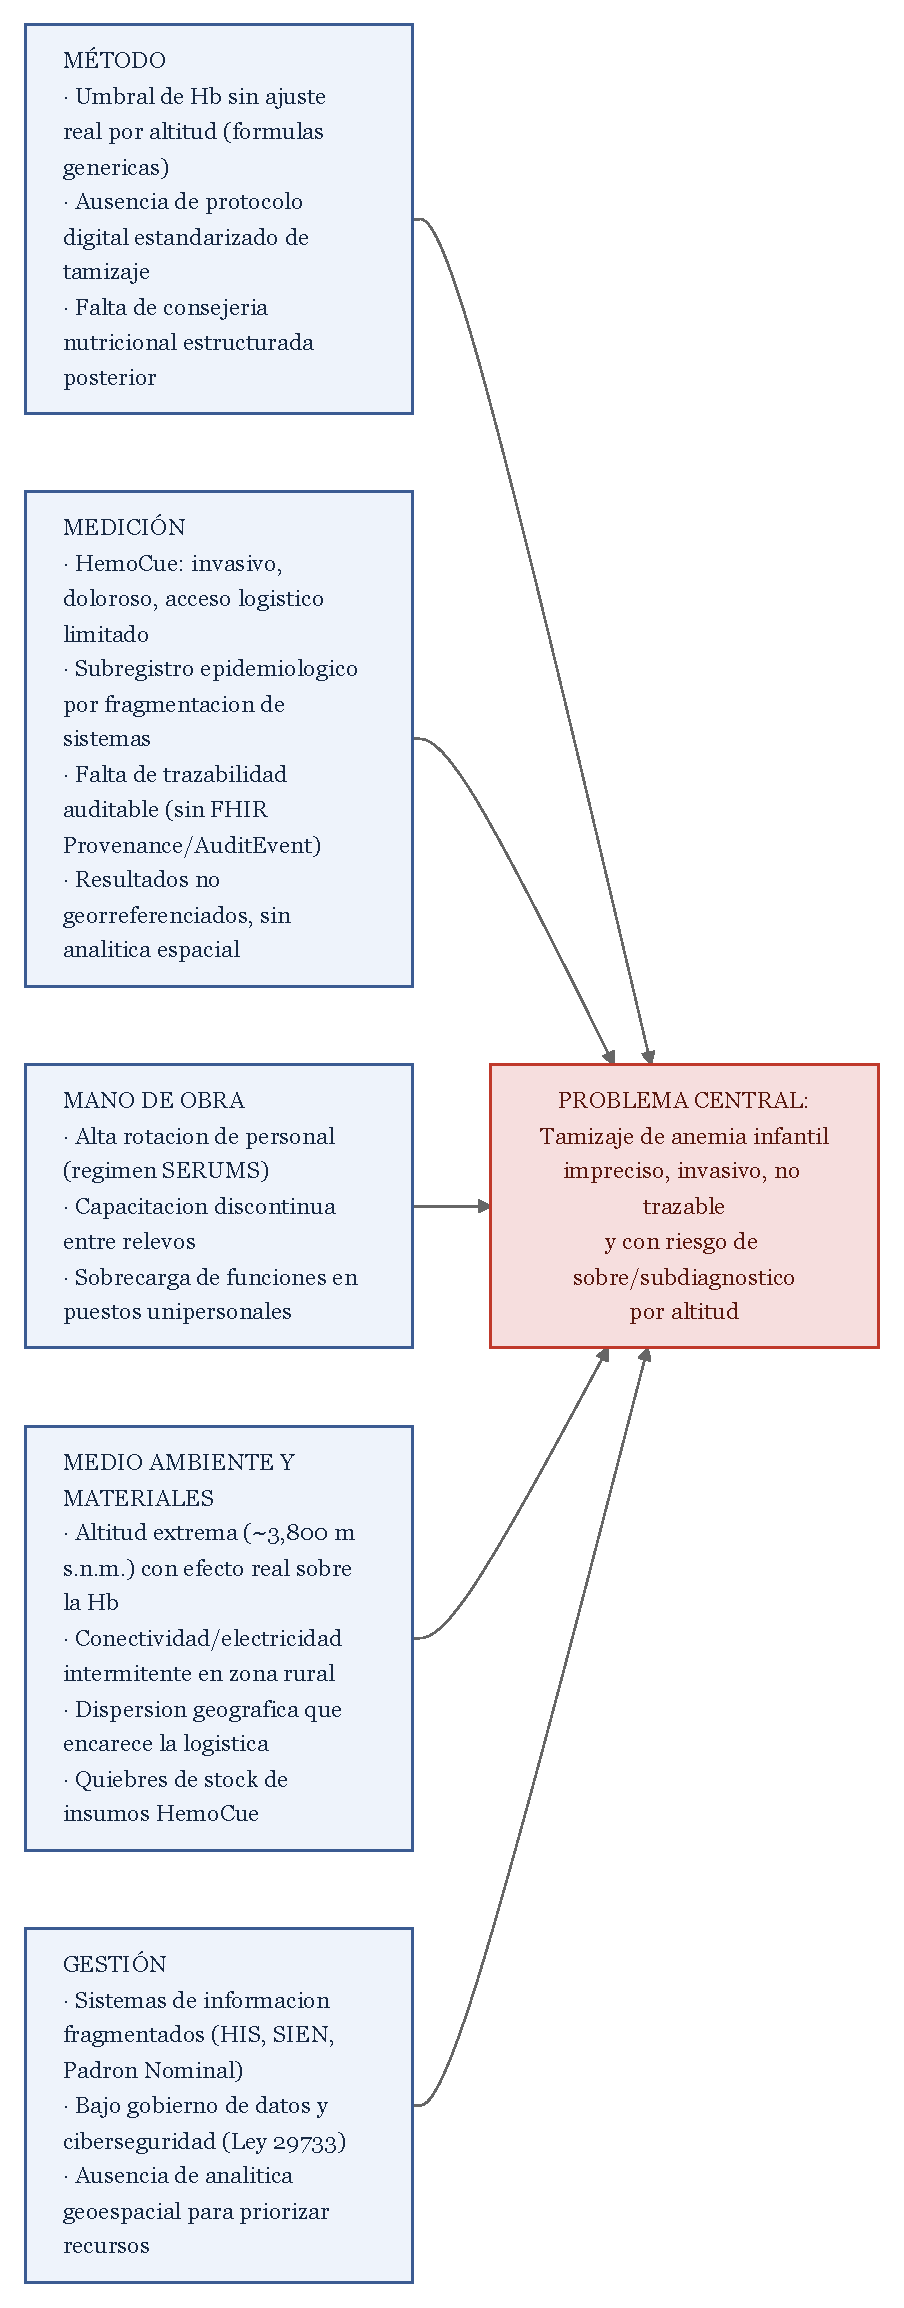
\includegraphics[width=0.7\linewidth,height=0.86\textheight,keepaspectratio]{assets/01-diagnostico/diagrama-03-ishikawa.pdf}
\caption*{Diagrama 3 --- Diagrama de causa-efecto (Ishikawa) de las causas raíz del problema central}
\end{figure}

De este análisis se desprende que las causas raíz no son homogéneas: algunas son de naturaleza \textbf{estructural/ambiental} (altitud, dispersión geográfica, conectividad), que HemoScan Andino no puede eliminar pero sí puede \textbf{compensar mediante diseño} (autocalibración por altitud, arquitectura offline-first); otras son de naturaleza \textbf{organizacional/gestión} (fragmentación de sistemas, bajo gobierno de datos), que HemoScan Andino puede \textbf{mitigar mediante interoperabilidad estándar} (FHIR); y otras son de naturaleza \textbf{operativa/humana} (rotación de personal, capacitación discontinua), que exceden el alcance de una solución tecnológica y requieren complementarse con estrategias de gestión del cambio y capacitación, a desarrollar en entregables posteriores (plan de gestión, roadmap tecnológico).

\subsubsection{1.4.3 Impacto estratégico}\label{impacto-estratuxe9gico}

El problema identificado tiene un impacto estratégico que trasciende el nivel operativo de la microred ilustrativa y se proyecta en al menos cuatro niveles:

\textbf{Nivel de política pública nacional y regional.} La anemia infantil no tratada oportunamente está asociada, según amplia evidencia científica internacional de dominio público en salud pública, a efectos adversos en el desarrollo cognitivo y motor infantil, con implicancias de largo plazo en el capital humano regional. Puno es la región con mayor prevalencia del país (56.1 \%, ENDES 2025), lo que convierte a este problema en un factor crítico de rezago frente a las metas del Plan Nacional Concertado de Salud y de los Objetivos de Desarrollo Sostenible, en particular el ODS 3 (Salud y Bienestar) y, de manera indirecta, el ODS 2 (Hambre Cero) y el ODS 10 (Reducción de las Desigualdades), dado el carácter históricamente inequitativo de la brecha de anemia entre zonas urbanas y rurales altoandinas.

\textbf{Nivel de gestión institucional (GERESA/DIRESA y municipios).} El indicador de prevalencia de anemia infantil es objeto de seguimiento y rendición de cuentas de las autoridades regionales y locales de salud. Un sistema de tamizaje impreciso ---ya sea por subdiagnóstico (que oculta casos reales) o por sobrediagnóstico inducido por mala corrección de altitud (que satura innecesariamente la capacidad de atención y erosiona la confianza en el sistema)--- distorsiona la información sobre la cual se basan las decisiones de política y asignación presupuestal, con el consiguiente riesgo reputacional y de gestión para las autoridades responsables.

\textbf{Nivel de confianza social e intercultural.} Dado que la punción capilar es percibida como un procedimiento invasivo y potencialmente doloroso para el menor, su uso repetido en tamizajes de seguimiento puede generar rechazo por parte de cuidadores, con el consecuente riesgo de abandono del control de Crecimiento y Desarrollo (CRED). Este riesgo de deserción del tamizaje tiene un impacto estratégico directo en la cobertura poblacional efectiva de cualquier programa de lucha contra la anemia, independientemente de la calidad clínica del método empleado.

\textbf{Nivel regulatorio y de responsabilidad legal.} La entrada en vigor del DS 115-2025-PCM y de la Ley N.° 29733 eleva el estándar exigido a cualquier sistema ---tecnológico o no--- que procese datos de salud de menores de edad o incorpore componentes de inteligencia artificial. Una microred que no adecúe sus procesos de tamizaje a estos estándares de trazabilidad y supervisión humana enfrenta un riesgo legal y reputacional creciente, independientemente de si adopta o no una solución como HemoScan Andino, lo que refuerza la relevancia estratégica de abordar esta brecha de manera proactiva.

\subsubsection{1.4.4 Justificación de la intervención}\label{justificaciuxf3n-de-la-intervenciuxf3n}

La intervención propuesta por HemoScan Andino se justifica en la medida en que atiende de manera directa y trazable cada una de las causas raíz identificadas en la sección 1.4.2, sin pretender ---y esto es una precisión deliberada y no una limitación menor--- sustituir el criterio clínico ni operar de forma autónoma:

\begin{itemize}
\tightlist
\item
  Frente a la causa de \textbf{método invasivo y de acceso limitado} (categoría Medición), HemoScan Andino propone la fusión de tres señales ópticas no invasivas de bajo costo (imagen de conjuntiva palpebral, espectrometría AS7341 de 11 canales, fotopletismografía MAX30102), reduciendo la dependencia exclusiva de la punción capilar.
\item
  Frente a la causa de \textbf{ausencia de corrección de altitud auditable} (categoría Método), se incorpora una capa de autocalibración por altitud basada en GPS combinado con un Modelo Digital de Elevación ---nunca altitud cruda de GPS---, que ajusta de forma transparente y auditable el umbral de hemoglobina, atendiendo directamente la advertencia de Gonzales et al.~(2025) y Baquerizo-Sedano et al.~(2025) sobre el riesgo de sobrediagnóstico por corrección inadecuada.
\item
  Frente a la causa de \textbf{conectividad y electricidad intermitentes} (categoría Medio ambiente), la arquitectura offline-first con inferencia embebida (ONNX/TFLite) en el propio dispositivo garantiza operatividad sin dependencia de conexión permanente.
\item
  Frente a la causa de \textbf{fragmentación de sistemas de información} (categoría Gestión), la trazabilidad basada en recursos FHIR (Observation, Provenance, AuditEvent, Consent, Device, Patient) y la interoperabilidad prevista con el HIS-MINSA y el Padrón Nominal atienden directamente la brecha de interoperabilidad diagnosticada en la sección 1.3.
\item
  Frente a la causa de \textbf{ausencia de analítica geoespacial} (categoría Gestión), el mapa de cobertura y riesgo geoespacial (MapLibre GL JS, PMTiles, H3, con técnicas analíticas como Getis-Ord Gi*, LISA, SaTScan y GWR/MGWR) provee a la Jefatura de microred y a la DIRESA una herramienta de priorización de recursos ausente en el estado actual.
\item
  Frente a la causa de \textbf{bajo gobierno de datos y riesgo normativo} (categorías Gestión y Medio ambiente regulatorio), la autenticación mediante Keycloak (OIDC, RBAC) y el diseño explícito orientado al cumplimiento de la Ley N.° 29733 y del DS 115-2025-PCM constituyen respuestas estructurales, no accesorias, al riesgo regulatorio identificado.
\end{itemize}

Es fundamental reiterar que HemoScan Andino se concibe como un \textbf{sistema de tamizaje que deriva a confirmación clínica, nunca como un diagnóstico autónomo}, en estricta observancia del principio de supervisión humana exigido por el DS 115-2025-PCM para sistemas de inteligencia artificial en el sector salud. Esta precisión no es meramente formal: es la que permite que la intervención sea normativamente viable y clínicamente responsable.

Finalmente, la justificación de intervención se refuerza con un argumento de factibilidad: el equipo ya cuenta con un presupuesto definido para la Fase 0 de validación (hardware de 3 nodos S/ 900; insumos de validación HemoCue S/ 400; submuestra de ferritina y PCR S/ 600; servidor/nube por 8 meses S/ 320; impresión 3D S/ 120; movilidad/campo S/ 400; materiales de gestión S/ 100; contingencia del 10 \% S/ 284; \textbf{total S/ 3,124}), lo que demuestra que la propuesta no es solo conceptualmente pertinente, sino operativamente factible para un primer piloto acotado de 150-300 niños en una microred, antes de escalar hacia las fases posteriores de piloto pagado y escalamiento regional. El desarrollo financiero detallado de estas fases corresponde al Caso de Negocio (Entregable CE0113), del cual este diagnóstico constituye el fundamento organizacional y estratégico directo. De manera complementaria, el detalle de la arquitectura tecnológica, las fases de implementación y el plan de escalamiento de la infraestructura de TI que dan soporte técnico a los componentes descritos en esta sección corresponden al \textbf{Roadmap de Tecnología (Entregable CE0114)}, de modo que los tres entregables del Área de competencia GTI ---CE0111/CE0112 (este documento), CE0113 y CE0114--- quedan explícitamente trazables entre sí.

\begin{center}\rule{0.5\linewidth}{0.5pt}\end{center}

\section{Anexos}\label{anexos}

\begin{quote}
\textbf{Nota sobre extensión del documento (hallazgo de revisión adversarial).} Este documento contiene aproximadamente 10,800 palabras y varias tablas extensas (en particular, el mapa de 14 stakeholders de la sección 1.1.4 y la matriz FODA cruzada del Anexo E). Convertido a un documento Word/PDF con formato académico estándar (fuente 11-12 pt, interlineado 1.15-1.5, márgenes normales), se estima que ocuparía entre 18 y 24 páginas, lo que excede el rango de 12-18 páginas sugerido para este entregable. Esta observación no corresponde a ninguno de los tres criterios de la rúbrica de calificación (3 puntos), pero se declara aquí explícitamente por transparencia. Antes de la entrega final en Word/PDF, se recomienda: (a) trasladar el glosario extenso (Anexo A) y la matriz FODA cruzada (Anexo E) a un apéndice separado del cuerpo principal, y/o (b) condensar las tablas más extensas del cuerpo del documento ---en particular el mapa de 14 stakeholders (sección 1.1.4)--- sin eliminar las columnas de sustento/evidencia que respaldan el rigor del análisis.
\end{quote}

\subsection{Anexo A --- Glosario de términos y siglas}\label{anexo-a-glosario-de-tuxe9rminos-y-siglas}

{\small
\begin{longtable}[]{@{}
  >{\raggedright\arraybackslash}p{(\linewidth - 2\tabcolsep) * \real{0.5000}}
  >{\raggedright\arraybackslash}p{(\linewidth - 2\tabcolsep) * \real{0.5000}}@{}}
\toprule\noalign{}
\begin{minipage}[b]{\linewidth}\raggedright
Sigla / término
\end{minipage} & \begin{minipage}[b]{\linewidth}\raggedright
Definición
\end{minipage} \\
\midrule\noalign{}
\endhead
\bottomrule\noalign{}
\endlastfoot
ANEMIA (tamizaje) & Proceso de detección temprana de niveles bajos de hemoglobina, previo a la confirmación diagnóstica clínica \\
BLE & Bluetooth Low Energy, protocolo de comunicación inalámbrica de bajo consumo energético \\
CRED & Control de Crecimiento y Desarrollo del niño, servicio de salud preventivo del primer nivel de atención \\
DIRESA / GERESA & Dirección Regional de Salud / Gerencia Regional de Salud, instancia de gobierno regional responsable de la salud pública \\
ENDES & Encuesta Demográfica y de Salud Familiar, instrumento estadístico oficial del INEI \\
FHIR & Fast Healthcare Interoperability Resources, estándar internacional de interoperabilidad de datos clínicos \\
GWR / MGWR & Geographically Weighted Regression / Multiscale GWR, técnicas de regresión espacial para análisis geoespacial de salud \\
H3 & Sistema de indexación geoespacial jerárquico hexagonal, usado para agregación y visualización de datos territoriales \\
HIS-MINSA & Sistema de Información de Hospitales del Ministerio de Salud, aplicativo de registro de atenciones \\
LISA & Local Indicators of Spatial Association, indicadores locales de autocorrelación espacial \\
MDE & Modelo Digital de Elevación, representación digital de la altitud del terreno usada para corrección contextual de hemoglobina \\
msnm & Metros sobre el nivel del mar \\
NTS & Norma Técnica de Salud, instrumento normativo emitido por el MINSA \\
OIDC / RBAC & OpenID Connect / Role-Based Access Control, estándares de autenticación y control de acceso basado en roles \\
ONNX / TFLite & Open Neural Network Exchange / TensorFlow Lite, formatos de modelos de aprendizaje automático optimizados para inferencia embebida \\
Padrón Nominal & Registro nominal de niñas y niños menores de 6 años, gestionado de forma interinstitucional por MINSA, MEF y RENIEC \\
PEI & Plan Estratégico Institucional \\
PESEM & Plan Estratégico Sectorial Multianual \\
PMTiles & Formato de archivo para servir mapas vectoriales estáticos sin necesidad de servidor de teselas dedicado \\
SaTScan & Software de detección de conglomerados (clusters) espaciales y espacio-temporales \\
SERUMS & Servicio Rural y Urbano Marginal de Salud, régimen obligatorio de profesionales de salud recién egresados \\
SIEN & Sistema de Información del Estado Nutricional \\
SIGA & Sistema Integrado de Gestión Administrativa \\
SIS & Seguro Integral de Salud \\
REUNIS & Repositorio Único Nacional de Información en Salud \\
\end{longtable}
}

\subsection{Anexo B --- Fuentes y referencias}\label{anexo-b-fuentes-y-referencias}

\begin{itemize}
\tightlist
\item
  Encuesta Demográfica y de Salud Familiar (ENDES) 2025. Instituto Nacional de Estadística e Informática (INEI). Indicador de prevalencia de anemia infantil en menores de 3 años, región Puno (56.1 \%).
\item
  Gonzales, G. F. et al.~(2025). {[}DATO PENDIENTE DE VALIDAR: título completo del artículo, revista, volumen y DOI --- solo se cuenta con autor y año según el enunciado del proyecto{]}. Referencia sobre el riesgo de sobrediagnóstico de anemia por corrección inadecuada de hemoglobina en altitud.
\item
  Baquerizo-Sedano, L. et al.~(2025). {[}DATO PENDIENTE DE VALIDAR: título completo del artículo, revista, volumen y DOI --- solo se cuenta con autor y año según el enunciado del proyecto{]}. Referencia complementaria sobre el mismo riesgo de sobrediagnóstico por altitud.
\item
  Ministerio de Salud del Perú. \textbf{Norma Técnica de Salud N.° 213-MINSA/DGIESP-2024}, ``Prevención y control de la anemia por deficiencia de hierro en el niño y la niña, adolescentes, mujeres en edad fértil, gestantes y puérperas'', aprobada mediante Resolución Ministerial N.° 251-2024/MINSA (10 de abril de 2024) y modificada por la Resolución Ministerial N.° 429-2024/MINSA (19 de junio de 2024). Verificada contra fuente oficial: Plataforma Digital Única del Estado Peruano (gob.pe/minsa) y El Peruano (busquedas.elperuano.pe/dispositivo/NL/2277624-1 y /NL/2299099-1).
\item
  Presidencia del Consejo de Ministros del Perú. \textbf{Decreto Supremo N.° 115-2025-PCM}, que aprueba el Reglamento de la Ley N.° 31814, ``Ley que promueve el uso de la inteligencia artificial en favor del desarrollo económico y social del país'' (seis títulos, 36 artículos y seis disposiciones complementarias finales; publicado en El Peruano el 9 de septiembre de 2025; vigente desde el 22 de enero de 2026). Verificada contra fuente oficial: Plataforma Digital Única del Estado Peruano (gob.pe/institucion/pcm/normas-legales/7133522-115-2025-pcm) y El Peruano (busquedas.elperuano.pe/dispositivo/NL/2436426-1).
\item
  Congreso de la República del Perú. Ley N.° 29733, Ley de Protección de Datos Personales.
\item
  MINSA -- MEF -- RENIEC. Padrón Nominal de niñas y niños menores de 6 años (marco interinstitucional de referencia).
\end{itemize}

\textbf{Nota sobre verificación de fuentes (actualizada tras revisión adversarial contra la rúbrica):} las referencias a Gonzales et al.~(2025) y Baquerizo-Sedano et al.~(2025) se citan tal como fueron provistas en el enunciado del proyecto (autor y año), sin acceso directo a la ficha bibliográfica completa, y permanecen marcadas como \textbf{{[}DATO PENDIENTE DE VALIDAR{]}}. Se recomienda que el equipo, antes de la sustentación final o publicación de resultados, valide y complete estas referencias en formato APA con la fuente original. En contraste, la NTS 213-MINSA/DGIESP-2024 y el DS 115-2025-PCM ---citadas repetidamente a lo largo del documento como hechos normativos--- \textbf{sí fueron contrastadas contra fuente oficial} (El Peruano y la Plataforma Digital Única del Estado Peruano) durante esta revisión, confirmándose su número, alcance y vigencia exactos; por ello no requieren la marca de dato pendiente de validar, a diferencia de lo que ocurría antes de esta verificación, cuando se citaban con el mismo nivel de certeza que fuentes no contrastadas.

\subsection{Anexo C --- Ficha técnica de la organización ilustrativa}\label{anexo-c-ficha-tuxe9cnica-de-la-organizaciuxf3n-ilustrativa}

{\small
\begin{longtable}[]{@{}
  >{\raggedright\arraybackslash}p{(\linewidth - 4\tabcolsep) * \real{0.3333}}
  >{\raggedright\arraybackslash}p{(\linewidth - 4\tabcolsep) * \real{0.3333}}
  >{\raggedright\arraybackslash}p{(\linewidth - 4\tabcolsep) * \real{0.3333}}@{}}
\toprule\noalign{}
\begin{minipage}[b]{\linewidth}\raggedright
Campo
\end{minipage} & \begin{minipage}[b]{\linewidth}\raggedright
Valor (ilustrativo / referencial)
\end{minipage} & \begin{minipage}[b]{\linewidth}\raggedright
Nota
\end{minipage} \\
\midrule\noalign{}
\endhead
\bottomrule\noalign{}
\endlastfoot
Nombre & Microred de Salud Altiplano-Puno & Nombre ficticio construido para fines académicos \\
Tipo de organización & Microred de salud pública de primer nivel de atención & Dependiente de GERESA/DIRESA Puno \\
Ubicación referencial & Zona altiplánica de la región Puno & Representativa de la Red de Salud San Román o Red de Salud Puno \\
Altitud referencial & 3,800 m s. n.~m. & Dato explícito del enunciado del proyecto \\
N.° de establecimientos (ilustrativo) & 1 Centro de Salud (I-4, cabecera) + 6 Puestos de Salud (I-1/I-2) = 7 establecimientos & Construcción ilustrativa; {[}DATO PENDIENTE DE VALIDAR: número real de establecimientos de la microred que participe{]} \\
Población asignada (ilustrativa) & Orden de magnitud de miles de habitantes & {[}DATO PENDIENTE DE VALIDAR: cifra real, a obtener del Padrón Nominal o INEI{]} \\
Niños menores de 3 años en la jurisdicción (ilustrativo) & Orden de magnitud de cientos & {[}DATO PENDIENTE DE VALIDAR: cifra real de la microred que participe{]} \\
Referencia regional de contexto & Población de Puno: aprox. 1.2-1.4 millones de habitantes; niños menores de 3 años en la región: orden de 60,000-80,000 & Estimaciones referenciales de orden de magnitud, a validar con Padrón Nominal, INEI o ENDES; no confundir con las cifras propias de la microred ilustrativa \\
Alcance previsto del piloto de tesis (Fase 0) & 150-300 niños en 1 microred & Estimación referencial del proyecto, presupuesto asociado de S/ 3,124 \\
Idioma(s) predominante(s) & Español, quechua y/o aymara (según zona) & {[}DATO PENDIENTE DE VALIDAR: proporción real de hablantes por comunidad{]} \\
Comité de ética constituido & No existe a la fecha & Requisito previo obligatorio antes de trabajo de campo \\
Convenio institucional formalizado & No existe a la fecha & Requisito previo obligatorio antes de validación con datos reales \\
\end{longtable}
}

\subsection{Anexo D --- Índice de diagramas y figuras presentados en el cuerpo del documento}\label{anexo-d-uxedndice-de-diagramas-y-figuras-presentados-en-el-cuerpo-del-documento}

{\small
\begin{longtable}[]{@{}
  >{\raggedright\arraybackslash}p{(\linewidth - 4\tabcolsep) * \real{0.3333}}
  >{\raggedright\arraybackslash}p{(\linewidth - 4\tabcolsep) * \real{0.3333}}
  >{\raggedright\arraybackslash}p{(\linewidth - 4\tabcolsep) * \real{0.3333}}@{}}
\toprule\noalign{}
\begin{minipage}[b]{\linewidth}\raggedright
Figura
\end{minipage} & \begin{minipage}[b]{\linewidth}\raggedright
Descripción
\end{minipage} & \begin{minipage}[b]{\linewidth}\raggedright
Ubicación
\end{minipage} \\
\midrule\noalign{}
\endhead
\bottomrule\noalign{}
\endlastfoot
Diagrama 1 & Estructura organizacional jerárquica (MINSA -\textgreater{} GERESA/DIRESA -\textgreater{} Red de Salud -\textgreater{} Microred -\textgreater{} Establecimientos) & Sección 1.1.2 \\
Diagrama 2 & Cadena de valor del proceso de tamizaje y atención de la anemia infantil, con punto de inserción de HemoScan Andino & Sección 1.1.3 \\
Diagrama 3 & Diagrama de causa-efecto (Ishikawa) de las causas raíz del problema central & Sección 1.4.2 \\
\end{longtable}
}

\subsection{Anexo E --- Matriz FODA cruzada (estrategias FO, FA, DO, DA)}\label{anexo-e-matriz-foda-cruzada-estrategias-fo-fa-do-da}

\textbf{Estrategias FO (Fortalezas-Oportunidades): usar fortalezas para aprovechar oportunidades}

{\small
\begin{longtable}[]{@{}
  >{\raggedright\arraybackslash}p{(\linewidth - 4\tabcolsep) * \real{0.3333}}
  >{\raggedright\arraybackslash}p{(\linewidth - 4\tabcolsep) * \real{0.3333}}
  >{\raggedright\arraybackslash}p{(\linewidth - 4\tabcolsep) * \real{0.3333}}@{}}
\toprule\noalign{}
\begin{minipage}[b]{\linewidth}\raggedright
N.°
\end{minipage} & \begin{minipage}[b]{\linewidth}\raggedright
Estrategia
\end{minipage} & \begin{minipage}[b]{\linewidth}\raggedright
Relación FODA
\end{minipage} \\
\midrule\noalign{}
\endhead
\bottomrule\noalign{}
\endlastfoot
FO1 & Aprovechar el vínculo comunitario existente (F1) y la prioridad de política pública (O2) para posicionar el piloto de HemoScan Andino como una intervención de alto impacto y bajo riesgo político & F1 + O2 \\
FO2 & Capitalizar la experiencia del personal en protocolos CRED/HemoCue (F2) y el marco normativo NTS 213 (O1) para acelerar la capacitación y adopción del nuevo método de tamizaje & F2 + O1 \\
FO3 & Utilizar la alianza académica con la UPeU (O6) para fortalecer la validación clínica requerida por el marco de IA en salud (O3) & O6 + O3 \\
\end{longtable}
}

\textbf{Estrategias FA (Fortalezas-Amenazas): usar fortalezas para mitigar amenazas}

{\small
\begin{longtable}[]{@{}
  >{\raggedright\arraybackslash}p{(\linewidth - 4\tabcolsep) * \real{0.3333}}
  >{\raggedright\arraybackslash}p{(\linewidth - 4\tabcolsep) * \real{0.3333}}
  >{\raggedright\arraybackslash}p{(\linewidth - 4\tabcolsep) * \real{0.3333}}@{}}
\toprule\noalign{}
\begin{minipage}[b]{\linewidth}\raggedright
N.°
\end{minipage} & \begin{minipage}[b]{\linewidth}\raggedright
Estrategia
\end{minipage} & \begin{minipage}[b]{\linewidth}\raggedright
Relación FODA
\end{minipage} \\
\midrule\noalign{}
\endhead
\bottomrule\noalign{}
\endlastfoot
FA1 & Usar el vínculo comunitario y la experiencia previa del personal (F1, F2) para gestionar la resistencia cultural al cambio (A3) mediante consejería y comunicación intercultural & F1 + F2 + A3 \\
FA2 & Apalancar la alineación con la política pública prioritaria (F5) para sostener el patrocinio institucional pese a eventuales cambios de gestión regional (A2) & F5 + A2 \\
\end{longtable}
}

\textbf{Estrategias DO (Debilidades-Oportunidades): superar debilidades aprovechando oportunidades}

{\small
\begin{longtable}[]{@{}
  >{\raggedright\arraybackslash}p{(\linewidth - 4\tabcolsep) * \real{0.3333}}
  >{\raggedright\arraybackslash}p{(\linewidth - 4\tabcolsep) * \real{0.3333}}
  >{\raggedright\arraybackslash}p{(\linewidth - 4\tabcolsep) * \real{0.3333}}@{}}
\toprule\noalign{}
\begin{minipage}[b]{\linewidth}\raggedright
N.°
\end{minipage} & \begin{minipage}[b]{\linewidth}\raggedright
Estrategia
\end{minipage} & \begin{minipage}[b]{\linewidth}\raggedright
Relación FODA
\end{minipage} \\
\midrule\noalign{}
\endhead
\bottomrule\noalign{}
\endlastfoot
DO1 & Aprovechar el abaratamiento de módulos BLE y smartphones (O5) para diseñar una arquitectura offline-first que compense la debilidad de conectividad intermitente (D2) & O5 + D2 \\
DO2 & Utilizar el marco regulatorio de IA auditable (O3) como guía de diseño para superar el bajo gobierno de datos actual (D6), convirtiendo el cumplimiento normativo en ventaja diferenciadora & O3 + D6 \\
\end{longtable}
}

\textbf{Estrategias DA (Debilidades-Amenazas): acciones defensivas para minimizar debilidades y amenazas simultáneamente}

{\small
\begin{longtable}[]{@{}
  >{\raggedright\arraybackslash}p{(\linewidth - 4\tabcolsep) * \real{0.3333}}
  >{\raggedright\arraybackslash}p{(\linewidth - 4\tabcolsep) * \real{0.3333}}
  >{\raggedright\arraybackslash}p{(\linewidth - 4\tabcolsep) * \real{0.3333}}@{}}
\toprule\noalign{}
\begin{minipage}[b]{\linewidth}\raggedright
N.°
\end{minipage} & \begin{minipage}[b]{\linewidth}\raggedright
Estrategia
\end{minipage} & \begin{minipage}[b]{\linewidth}\raggedright
Relación FODA
\end{minipage} \\
\midrule\noalign{}
\endhead
\bottomrule\noalign{}
\endlastfoot
DA1 & Priorizar la validación clínica rigurosa de la corrección por altitud (mitigando D5) antes de cualquier escalamiento, para prevenir que un algoritmo mal calibrado materialice el riesgo de sobrediagnóstico (A5) y erosione la confianza institucional & D5 + A5 \\
DA2 & Diseñar mecanismos de consentimiento y trazabilidad digital desde el inicio (mitigando D6) para anticipar el riesgo regulatorio de la Ley 29733 (A4), en lugar de remediarlo de forma reactiva & D6 + A4 \\
\end{longtable}
}

\begin{center}\rule{0.5\linewidth}{0.5pt}\end{center}

\section{Autoevaluación frente a la rúbrica}\label{autoevaluaciuxf3n-frente-a-la-ruxfabrica}

\emph{(Sección actualizada tras una verificación adversarial de este documento contra la rúbrica oficial; las calificaciones y justificaciones que siguen reemplazan una versión anterior más optimista.)}

{\small
\begin{longtable}[]{@{}
  >{\raggedright\arraybackslash}p{(\linewidth - 4\tabcolsep) * \real{0.3333}}
  >{\raggedright\arraybackslash}p{(\linewidth - 4\tabcolsep) * \real{0.3333}}
  >{\raggedright\arraybackslash}p{(\linewidth - 4\tabcolsep) * \real{0.3333}}@{}}
\toprule\noalign{}
\begin{minipage}[b]{\linewidth}\raggedright
Criterio
\end{minipage} & \begin{minipage}[b]{\linewidth}\raggedright
Nivel alcanzado
\end{minipage} & \begin{minipage}[b]{\linewidth}\raggedright
Justificación
\end{minipage} \\
\midrule\noalign{}
\endhead
\bottomrule\noalign{}
\endlastfoot
Análisis del contexto organizacional & \textbf{Bueno} & El análisis integra fuentes citadas (ENDES 2025, literatura sobre altitud, marco normativo NTS 213/DS 115-2025-PCM/Ley 29733) y frameworks estructurados (cadena de valor, mapa de 14 stakeholders, estructura organizacional en cuatro niveles). Sin embargo, la organización diagnosticada, ``Microred de Salud Altiplano-Puno'', es explícitamente ficticia/ilustrativa (declarado en la nota metodológica y en el Anexo C): no existe convenio real, y los datos organizacionales específicos (número de establecimientos, población, estructura interna detallada) son construcciones del propio equipo, no evidencia primaria de una organización real. La rúbrica exige, para ``Excelente'', un análisis ``con evidencia y sustento estratégico'' de una organización real; al faltar esa evidencia primaria, el criterio no alcanza el nivel ``Excelente'' pleno, y se califica honestamente como \textbf{Bueno}. \\
Identificación de brechas estratégicas & \textbf{Bueno} & Se identifican 15 brechas tecnológicas y \textbf{24 factores FODA} (5 fortalezas, 7 debilidades, 6 oportunidades y 6 amenazas --- corregido en esta revisión; una versión anterior de este documento citaba erróneamente ``20 factores'' en el Resumen Ejecutivo y en esta misma tabla, un error de conteo ya subsanado), cada uno con una columna explícita de sustento/evidencia, además de una matriz de síntesis (1.2.5) que conecta objetivos estratégicos con brechas concretas. La evaluación de madurez digital (1.3.2) fue además corregida en esta revisión para usar exclusivamente valores puntuales (no rangos) dentro de su escala ordinal de 5 niveles, eliminando una inconsistencia de escala detectada. Pese a estas correcciones, el criterio no alcanza ``Excelente'' pleno porque las brechas se derivan de diagnóstico documental y de un juicio profesional ilustrativo del equipo, no de un instrumento de evaluación de madurez digital aplicado formalmente a una microred real; ese sería el siguiente paso una vez exista convenio institucional. \\
Alineamiento estratégico del proyecto & \textbf{Excelente} & El documento traza una cadena explícita y verificable entre el problema (prevalencia de anemia, limitaciones del HemoCue, riesgo de sobrediagnóstico por altitud), los objetivos estratégicos institucionales formulados (OE1-OE5), las causas raíz (diagrama de Ishikawa) y cada componente técnico de la propuesta de HemoScan Andino (sección 1.4.4), evidenciando coherencia de principio a fin. En esta revisión se reforzó además la trazabilidad explícita con el Caso de Negocio (Entregable 2, CE0113), sin que se hayan detectado vacíos de contenido mínimo en este eje. Nota de alcance: el Roadmap de Tecnología (CE0114) y la Matriz de Riesgos Estratégicos (CE0115), aunque se listan como evidencia de la competencia CE011 en el resumen oficial del área, no constituyen un entregable formal separado dentro del alcance de Semestre 1 acordado para este proyecto; sus elementos quedan parcialmente cubiertos por el registro de riesgos del Business Case (Entregable 2, sección 2.5) y del Plan de Gestión (Entregable 3, sección 3.5), y se registran como una extensión pendiente de este diagnóstico. \\
\end{longtable}
}

\textbf{Limitación transversal declarada:} el nivel ``Excelente'' pleno en los dos primeros criterios requiere, como condición necesaria, información primaria de una microred real (entrevistas con la Jefatura y el personal de salud, datos oficiales de población y establecimientos, un instrumento formal de evaluación de madurez digital, y la constitución de un comité de ética). Ninguno de estos insumos existe a la fecha de este diagnóstico, por lo que se han declarado explícitamente como \textbf{{[}DATO PENDIENTE DE VALIDAR{]}} a lo largo del documento, en lugar de presentarse como hallazgos verificados.

\textbf{Rigor de citas normativas/académicas (hallazgo transversal, verificado en esta revisión):} las citas académicas incompletas (Gonzales et al., 2025; Baquerizo-Sedano et al., 2025) ya estaban correctamente marcadas como \textbf{{[}DATO PENDIENTE DE VALIDAR{]}}. En esta revisión se verificaron adicionalmente, contra fuente oficial (El Peruano y la Plataforma Digital Única del Estado Peruano), las dos normas centrales que el documento citaba repetidamente como hechos sin el mismo tratamiento de validación: la \textbf{NTS 213-MINSA/DGIESP-2024} (aprobada por RM N.° 251-2024/MINSA, modificada por RM N.° 429-2024/MINSA) y el \textbf{DS 115-2025-PCM} (reglamento de la Ley N.° 31814, publicado el 9 de septiembre de 2025, vigente desde el 22 de enero de 2026). Ambas resultaron ser normas reales y vigentes, con el número y alcance citados correctamente en el cuerpo del documento; el detalle de verificación se añadió al Anexo B. De haber resultado no verificables, se habrían marcado con la misma etiqueta \textbf{{[}DATO PENDIENTE DE VALIDAR{]}} usada para las demás fuentes no contrastadas, en vez de mantenerlas como hechos asumidos.

\textbf{Formato sugerido (extensión):} se detectó y declaró explícitamente, en una nota al inicio de la sección de Anexos, que la extensión estimada del documento (18-24 páginas en formato Word/PDF estándar) excede el rango sugerido de 12-18 páginas. Este hallazgo no forma parte de los tres criterios de la rúbrica de 3 puntos, pero se registra aquí por completitud y se ofrecen recomendaciones concretas de condensación antes de la entrega final.


\end{document}
